\chapter{Introduction}\label{chap:intro}


%\textit{While the majority of this chapter was written for the thesis, parts of Sec \ref{sec:astero_intro} were written for \cite{2017North} and have been adapted from the introduction in that work to limit repetition. \textbf{YOU WANT SOMETHING LIKE THIS AT THE START OF EACH SCIENCE CHAPTER TOO, TO SHOW WHAT YOU DID AND ANY ACKNOWLEDGEMENTS OF OTHER PEOPLE}}

\glsresetall 
{}
%%%%%%%%%%%%%%%%%%%%%%%%%%%%%%%%%%%%%%%%%%%%%%%%%%%%%%%%%%%%%%%%%%%%%%%%
%%%%%%%%%%%%%%%%%%%%%%%%%%%%%%%%%%%%%%%%%%%%%%%%%%%%%%%%%%%%%%%%%%%%%%%%
%%%%%%%%%%%%%%%%%%%%%%%%%%%%%%%%%%%%%%%%%%%%%%%%%%%%%%%%%%%%%%%%%%%%%%%%
\section{Solar Activity}\label{sec:intro_activity}

%%%%%%%%%%%%%%%%%%%%%%%%%%%%%%%%%%%%%%%%%%%%%%%%%%%%%%%%%%%%%%%%%%%%%%%%
\subsection{Background}

Solar activity varies periodically, with a duration of approximately 11 years, known as the solar cycle \citep{hathaway_solar_2015}. The solar cycle is a magnetic effect and is driven by the Sun's dynamo processes. Magnetic fields and the ionised plasma in the Sun's interior move together, as the magnetic field is `frozen' to the plasma; thermonuclear reactions and the inductive action of plasma occur in the Sun's core, giving rise to complex structures and dynamics in the outer layers of the Sun \citep{charbonneau_dynamo_2020}.

It is well known that the 11-year solar activity cycle is in fact a 22-year cycle -- the Hale cycle -- which describes the alternating polarity and the full regeneration of the large-scale solar magnetic field \citep{hathaway_solar_2015, charbonneau_dynamo_2020}. The Sun's large-scale magnetic field alternates between a poloidal field and a toroidal field \citep{charbonneau_dynamo_2020}, i.e. following the sequence:

\begin{equation}
P(+) \rightarrow T \rightarrow \textcolor{blue}{P(-) \rightarrow T \rightarrow} \textcolor{orange}{P(+) \rightarrow T \rightarrow} ... \, ,
%P(+) \rightarrow T(-) \rightarrow P(-) \rightarrow T(+) \rightarrow P(+) \rightarrow ... \, ,
\label{eq:solar_cycle_dynamo}
\end{equation}
%
where the $P$ and $T$ refer to poloidal and toroidal fields, respectively, $(+)$ and $(-)$ refer to the signs of the poloidal field polarity, and each colour denotes a complete 22-year Hale cycle.

Starting with a poloidal field with positive polarity, $P(+)$, differential rotation causes shearing of the magnetic field and it wraps around the Sun. As a result the magnetic field becomes concentrated at certain latitudes above and below the equator. This is named the $\Omega$-effect and is the creation of a toroidal field with opposite polarity to the poloidal field, $T(-)$ \citep{hathaway_solar_2015}.

The recovery of the poloidal field with the same polarity as the toroidal field, $P(-)$, is the $\alpha$-effect, but the details of how this effect works in the Sun is less well understood \citep{hathaway_solar_2015}. Helical motions that lift and twist the magnetic field which are important in the $\alpha$-effect \citep{babcock_topology_1961} and result from such processes as: (i) turbulence and mean-field electrodynamics; (ii) the Babcock-Leighton mechanism; (iii) hydrodynamical and magnetohydrodynamical instabilities (see \citet{charbonneau_dynamo_2020} for a complete review). This underpins the re-creation of a poloidal field with the same polarity as the toroidal field, $P(-)$. This process repeats with each cycle from poloidal field to poloidal field (i.e. $P(+)\rightarrow P(-)$) taking $\sim11$~years, and hence $\sim22$~years for the full magnetic cycle, the Hale cycle, to regenerate a poloidal field with the same polarity (i.e. $P(+)\rightarrow P(+)$).%(d) and (e) show the effect of cyclonic turbulence on former toroidal fields, creating small-scale secondary poloidal magnetic fields - the α-effect. Averaged, they result in a net electromotive force generating a new large-scale poloidal field(f), closing the first half part of the magnetic cycle with a new poloidal field (g), with opposite polarity than the initial one. (h)represents the beginning of the Babcock-Leighton mechanism: toroidal flux tubes buoyantly rise to the surface forming sunspots, tilted bipolar regions. In (i), the fields from the bipolar regions diffuse and reconnect with each other and with the polar fields. The resulting poloidal flux is advected by meridional circulation to the poles (j), generating the final large-scale poloidal field in (g). 


The earliest observations of solar activity and the solar cycle were of sunspots, which date back to over 2000 years ago \citep{clark_interpretation_1978}. Sunspots are dark regions of concentrated, active magnetic flux which cross the photosphere. The earliest observation of a solar cycle dependence on sunspots was by \citet{schwabe_sonnenbeobachtungen_1844}, who stated that annual observations of sunspot groups, over a duration 18~years from 1826--1844, showed a cyclic behaviour, with a period of about 10 years.

Following this discovery \citet{wolf_extract_1859} acquired daily observations of \glspl{ssn} and extended the records as far back as 1749 \citep{hathaway_solar_2015}. This used a method of estimating the individual sunspots from identify group of sunspots and these \glspl{ssn} have been used to monitor the solar activity cycle since \citep{wolf_extract_1859, wolf_abstract_1861}. Each activity cycle has unique characteristics; however, common among all cycle is that the sunspot numbers have been used to measure the minimum and maximum of the cycle, as we can see in Figure~\ref{fig:ssn}, for sunspot observations dating back to the year $\sim1750$.

\begin{figure}[ht!]
	\centering
	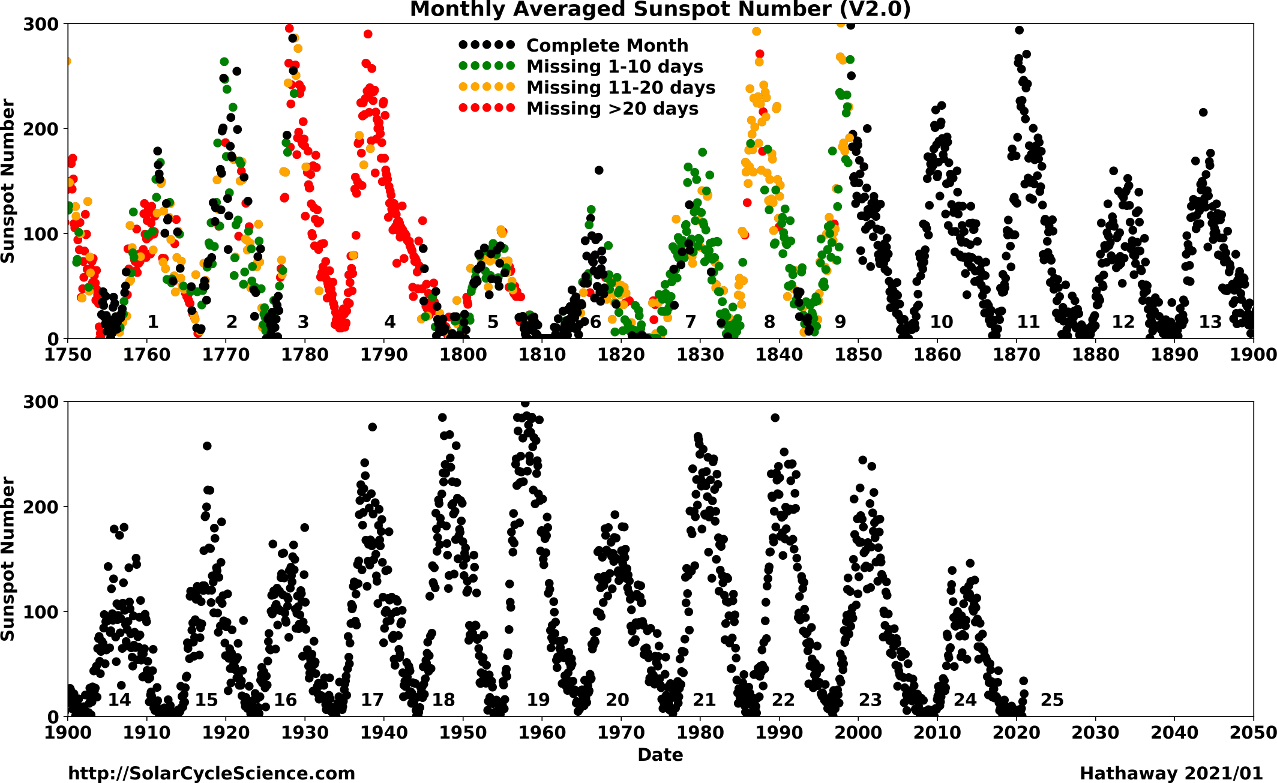
\includegraphics[width=\columnwidth]{SSN_monthly_landscape.png}
	\caption{Monthly averaged sunspot number since 1750 \citep{hathaway_solar_2017}. Black points indicate a full month of data, and then a traffic light system is in place to represent data quality, i.e. green for a near-complete month of data, amber for near 50\% duty cycle, and red for a very low data duty cycle.}
	\label{fig:ssn}
\end{figure}

Observations of sunspots in the 17th Century allowed astronomers to accurately measure the rotation of the Sun's surface, which they measured to be slightly under four weeks \citep{casanovas_early_1997, casas_solar_2006, luminet_reception_2017}. These early observations also showed that sunspots did not appear at latitudes higher than $\sim29^{\circ}/30^{\circ}$ \citep{casanovas_early_1997}. Later, it was confirmed that regions of strong surface magnetic activity was not distributed uniformly over the solar surface and also that the Sun exhibited a latitude-dependent differential surface rotation \citep{lee_cyril_1858}. %At the start of each cycle spots appear at latitudes above about $20^{\circ}-25^{\circ}$. 

As the solar cycle evolves the range of latitudes displaying sunspots increases and the typical latitude of spots slowly drifts towards the equator, with a zone of avoidance near the equator \citep{hathaway_solar_2015}. This behaviour was first noticed by \citet{carrington_observations_1863} and is known as Sp\"{o}rer’s Law of Zones, illustrated by the ``Butterfly Diagram" \citep{maunder_spoerers_1903, maunder_note_1904}, see Figure~\ref{fig:butterfly}.

\begin{figure}[ht!]
	\centering
	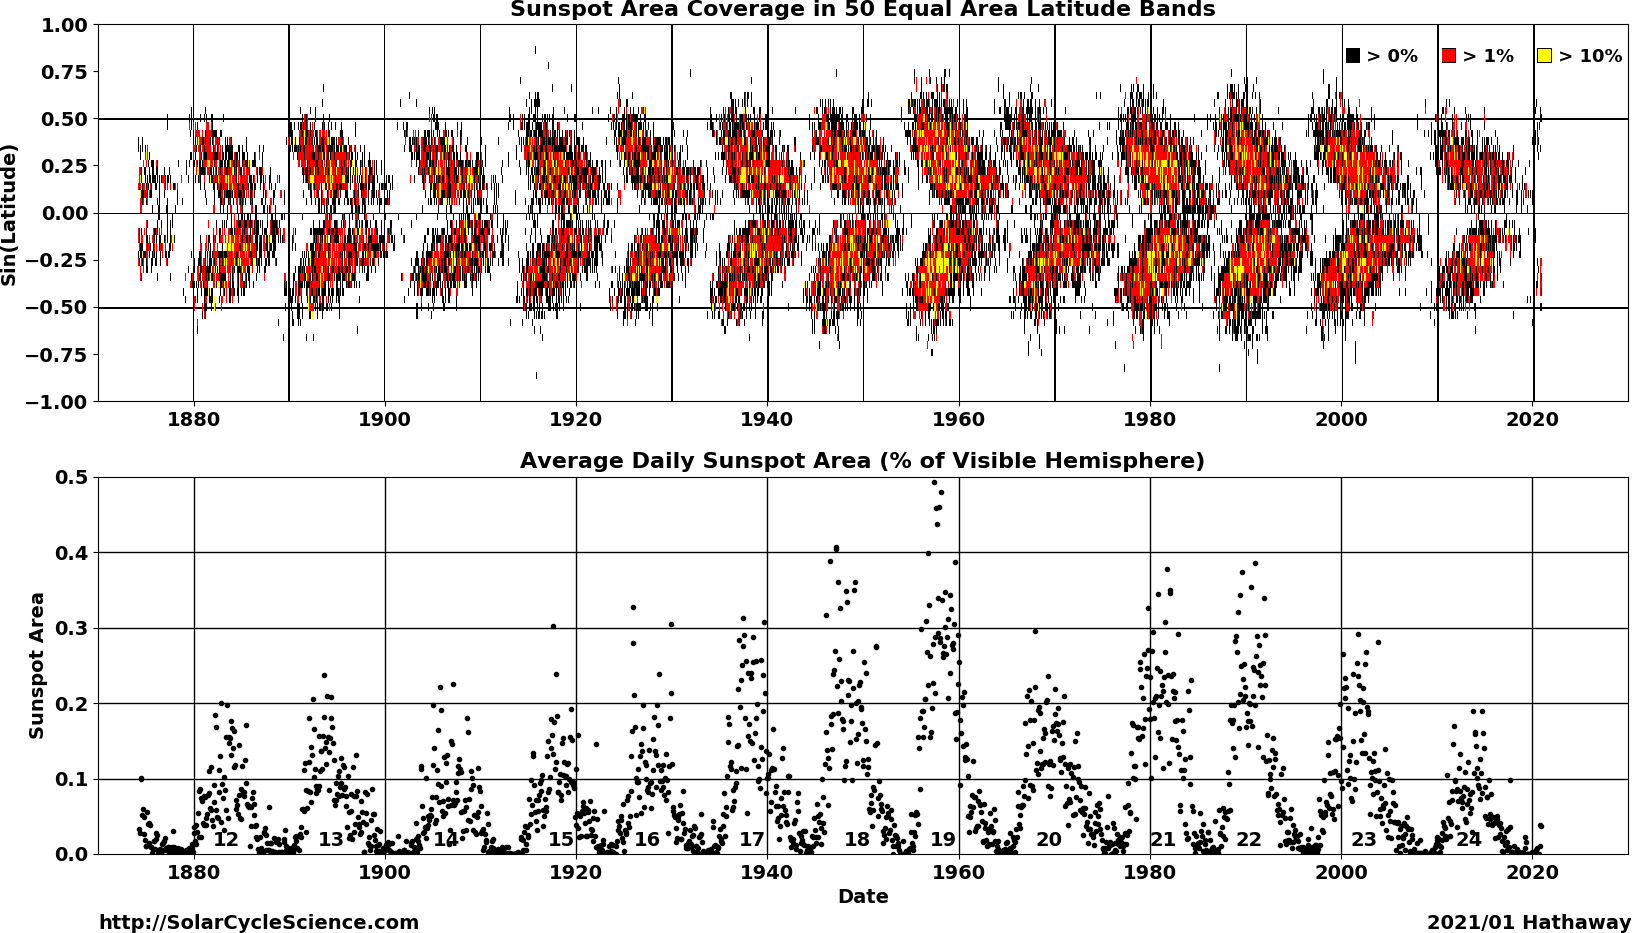
\includegraphics[width=\columnwidth]{ButterflyDiagram.png}
	\caption{Top panel: shows the latitudinal distribution of sunspots over time (also known as a ``Butterfly Diagram") and the colour of the points depict the area of the disc. Bottom panel: shows the average daily area of sunspots on the visible solar disc. Taken from \citet{hathaway_solar_2017}.}
	\label{fig:butterfly}
\end{figure}

In the first half of the 20th Century, it was discovered that sunspot groups in both hemispheres were tilted with respect to the Sun's equator, such that the leading spots exist closer to the equator than the following spots. This was first published in \citet{hale_magnetic_1919} but later defined as Joy's law. Furthermore, the degree of tilt varies with latitude, with a larger tilt at higher latitudes, and the tilt varies with the solar cycle \citep{hathaway_solar_2015}. In addition, sunspots groups also have opposite polarities in the Northern to Southern hemispheres, and the polarity changes from cycle-to-cycle. This effect is known as Hale’s Polarity Law \citep{hale_law_1925}.

With the invention of the magnetograph \citep{babcock_solar_1953}, the Sun's magnetic field was probed further and it was discovered that sunspots were only the tip of the iceberg. It was discovered that sunspots are a small part of larger \glspl{ar} of magnetic field, which may be both \glspl{bmr} or \glspl{umr} \citep{babcock_suns_1955}.

Joy's law implies that the tilt of \glspl{bmr} systematically places the leading-polarity-flux at a lower latitude than the following-polarity-flux \citep{hathaway_solar_2015}. It is believed that there is a cancellation of leading-polarity flux on opposite hemisphere near the equator \citep{dasi-espuig_sunspot_2010}. Poleward transport of following-polarity-flux by diffusion and the meridional flow is responsible for the reversal of the polar field polarity after a toroidal field (see equation~\ref{eq:solar_cycle_dynamo}) \citep{sheeley_surface_2005, charbonneau_dynamo_2020}.

In very modern literature, the definition of the solar activity cycle has started to deviate away from counting sunspots and instead tracking the magnetic activity bands over the full, 22-year, Hale cycle \citep{leamon_termination_2018, leamon_timing_2020}. The existence of a ``Terminator" has been shown, which marks the hand-over from one solar cycle to the next \citep{mcintosh_deciphering_2014, mcintosh_what_2019}. The terminator is defined as the abrupt annihilation or cancellation event of the oppositely polarized magnetic activity bands from at the solar equator \citep{mcintosh_what_2019}. By employing the Hilbert transform to different proxies of the solar cycle \citet{leamon_timing_2020} demonstrated a robust method to identify and predict the signature of terminators. Since, the method has been used to map severe space weather events to a ``solar cycle phase clock" \citep{chapman_quantifying_2020} and forecast the properties of Solar Cycle 25 \citep{mcintosh_overlapping_2020}. There exists some uncertainty about terminators in the solar physics community, but the evidence presented so far suggests this method is robust, but will ultimately be tested with the evolution of Solar Cycle 25.


As discussed, the solar activity cycle exhibits a clear periodicty of approximately 11~years; however, there exists other, short-term periodicities in the solar activity cycle (see \citet{hathaway_solar_2015} for a review). The most prominent other feature in the solar activity cycle is a $\sim2$-year periodicity which manifests as a double peak in the maximum of \gls{ssn}, known as the Gnevyshev gap \citep{gnevyshev_corona_1963, gnevyshev_11-years_1967}. It was thought that this phenomena was due to a superposition of sunspots from both hemispheres, slightly out of phase, but it was later confirmed that the Gnevyshev gap occurs in each hemisphere separately \citep{norton_solar-cycle_2009}. The cause of the Gnevyshev effect remains an open question \citep{hathaway_solar_2015}.

Finally, it has been suggested that long-term variations exist in the solar activity cycle, which consist of grand maxima and grand minima, which have led to the events such as the Maunder minimum (circa 1650--1700) and the Dalton minimum (circa 1790--1820). However, there is little evidence to support this long-term, cyclic variation \citep{hathaway_solar_2015}.

%[any discussion on peculiarities, such as large minima, i.e. maunder minimum, and recent extended deep minimum of cycle 23/24...?]


%%%%%%%%%%%%%%%%%%%%%%%%%%%%%%%%%%%%%%%%%%%%%%%%%%%%%%%%%%%%%%%%%%%%%%%%
\subsection{Features of Solar Activity}

There are many features that can be observed across the electromagnetic spectrum as a result of solar activity. In addition, with the advent of the magnetograph, solar activity can also be observed with direct measurements of the Sun's magnetic field, at different spatial scales. Many of these features are used widely in the literature as proxies of the solar activity cycle. Here we discuss these features and their properties.


\subsubsection*{Active Regions}

An \gls{ar} has been defined as all \textit{observable} magnetic phenomena that appears preceding, during, and following the birth of sunspots, including electromagnetic and \gls{sep} emission \citep{kiepenheuer_structure_1968}. However, more generally, they appear when strands of magnetic flux emerge into the visible atmosphere from the solar interior and through the surface of the Sun. 

\citet{van_driel-gesztelyi_evolution_2015} recently proposed a new and more accurate definition of \glspl{ar}:

\begin{quote}
	\textit{the totality of observable phenomena in a 3D volume represented by the extension of the magnetic field from the photosphere to the corona, revealed by emissions over a wide range of wavelengths accompanying and following the emergence of strong twisted magnetic flux (i.e. kG).}% The simplest \glspl{ar} have bipolar magnetic field configurations, but \glspl{ar} may be built-up by several bipoles emerging in close succession.}
\end{quote}

This definition does not hinge on the appearance of a sunspot, which is important as not all \glspl{ar} produce spots \citep{van_driel-gesztelyi_evolution_2015}, and clearly defines the conditions and features of \glspl{ar}. \glspl{ar} comprise of features in the photosphere, chromosphere, and corona; they typically appear as bipolar regions, obeying Hale's law, Joy's law, and Sp\"{o}rer’s Law, and display a wide range of sizes and lifetimes. In addition, \glspl{ar} are typically confined to the specific `active' bands of latitude, between $\pm40^{\circ}$ \citep{harvey_solar_2001}.

The \glspl{ar} which produce sunspots are typically 10--100~Mm in size and have lifetimes on the order of one to two months (i.e. one or two solar rotations) \citep{canfield_solar_2001}. However, it has been observed that \gls{ar} exist lifetimes in the range of days--months \citep{schrijver_solar_2008}. It is generally accepted that the lifetime of \glspl{ar} depend approximately linearly on their size and strength \citep{canfield_solar_2001, schrijver_solar_2008}. The end of an \gls{ar} is determined by the dispersal of the magnetic flux by convective motion, differential rotation, meridional flows, and magnetic reconnection \citep{canfield_solar_2001}.


There are several other features that arise out of \glspl{ar}, such as: faculae, plages, and networks. Faculae are bright spots visible in the photosphere that appear bright at the limb but are nearly invisible at disc centre. They arise due to small magnetic flux tubes creating pores in the photosphere \citep{solovev_structure_2019}. If the flux tubes are small enough, they are heated by horizontal radiation transfer maintaining the pressure and the walls appear brighter than the surrounding area, which is known as the `hot-wall' model \citep{spruit_pressure_1976, keller_origin_2004}. Plages are bright regions in the solar chromosphere and are the chromospheric counterparts of faculae \citep{pillet_active_1997}. Networks are a product of the decaying remnants of \glspl{ar}, the merging and cancelling of mixed polarity fields in and around \glspl{ar}, and ephemeral regions -- often referred to as the `salt and pepper' field \citep{martin_identification_1988}.


\subsubsection*{Ephemeral Regions}

A short-lived class of \glspl{ar} exists, known as \glspl{er} due to their short lifetimes.  \glspl{er} have sizes typically less than 20~Mm, lifetimes of a few hours, and produce no sunspots \citep{harvey_solar_2001}.

\glspl{er} emerge rapidly and it is possible that thousands of \glspl{er} emerge over the entire solar surface within a 24-hour period \citep{harvey_solar_2001}. There has been some disagreement in the literature on the temporal evolution of \glspl{er} with contradictory statements regarding whether the occurrence of \glspl{er} follows the activity cycle (see \citet{harvey_properties_1993, hagenaar_ephemeral_2001, vieira_evolution_2010}). However, some studies show compelling evidence that \glspl{er} are correlated with the solar activity cycle (see e.g. \citet{vieira_evolution_2010,chaplin_sensitivity_2019}, and references therein). It was also shown that \glspl{er} follow the solar activity cycle but with a slight shift in phase compared to the sunspot minimum \citep{harvey_ephemeral_1973, martin_ephemeral_1979}.

Unlike \glspl{ar}, \glspl{er} are spatially located all over the solar disc \citep{harvey_solar_2001}. Furthermore \glspl{er} at high latitudes have been interpreted to be the first emergence of bipolar regions associated with the onset of a new solar cycle. Despite these differences, it has been reported that it is difficult to differentiate between large \glspl{er} and small \glspl{ar} \citep{harvey_solar_2001}.



\subsubsection*{Sunspots}

As discussed above, sunspots have been used for centuries as a proxy for solar activity. Sunspots are dark regions on the disc of concentrated magnetic field. The convective heat flow is disrupted due to the magnetic field, therefore leaving the spots cooler than the surrounding photosphere \citep{solanki_sunspots_2003, hathaway_solar_2015}. Sunspots can sometimes appear in isolation; however, sunspots are generally found in groups, obeying Hale's law, Joy's law, and Sp\"{o}rer’s Law. Each sunspot
is characterised by a dark, central core, called the \textit{umbra}, and a halo, called the \textit{penumbra} \citep{howard_sunspot_2001, solanki_sunspots_2003}. Sunspot groups are an important photometric counterpart of \glspl{ar} as the locations of extreme solar activity such as flares and \glspl{cme}.

The sizes of sunspots can vary substantially from diameters of around 2000~km, for the smallest sunspots, up to 60~Mm or more \citep{howard_sunspot_2001,solanki_sunspots_2003}. The lifetimes of sunspots range from minutes to months \citep{howard_sunspot_2001, solanki_sunspots_2003} and \citet{howard_sunspot_2001} states that more than half of sunspots have lifetimes $<2$~days, $90\%$ of sunspots have lifetimes $<11$~days, and it is rare for sunspots to have lifetimes of more than a few months. The lifetime increases linearly with maximum size, following the Gnevyshev-Waldmeier rule \citep{gnevyshev_notitle_1938, waldmeier_ergebnisse_1955}. The largest spots are generally the survivors of large sunspot groups, appearing as a single spot at least in the later stage of their lifetime \citep{howard_sunspot_2001}.

The equatorward drift of sunspots is a well-known characteristics of the evolution of sunspots during the solar cycle. Sunspots emerge in active latitudes at around $\sim~25-30^{\circ}$, and as the cycle progresses the mean latitude of the spots in each hemisphere steadily decreases. The temporal distributions of sunspots shows more spots are observed at solar maximum and few observed at solar minimum (see Fig.~\ref{fig:ssn}). As such, the sunspot number is the most commonly used proxy for solar activity \citep{hathaway_solar_2015} and the \gls{issn} is the most widely used data set due to the length of the available record \citep{hathaway_solar_2015}. 

\glspl{ssn} are preserved and disseminated by the \gls{wdc} \gls{silso} of the Royal Observatory of Belgium \citep{silso_world_data_center_international_1954} and are provided as the daily \gls{ssn}, monthly averages, yearly averages, and the box-car smoothed \gls{ssn}. The standard smoothing is a 13-month \gls{cma} and the solar cycle maxima and minima are usually defined in terms of the smoothed \gls{ssn} \citep{hathaway_solar_2015}.



\subsubsection*{10.7 cm Flux}

The 10.7~cm solar flux (F$_{10.7}$) is the disc-integrated radio emission at a wavelength of 10.7~cm (in a 100~MHz‐wide band centred on 2800~MHz) from the Sun \citep{tapping_limits_1994,tapping_107_2013}. It is one of the most widely used indices of solar activity, alongside the \gls{ssn}, and the F$_{10.7}$ measure of solar activity has advantages over the \gls{ssn} in that it is completely objective \citep{hathaway_solar_2015}.

The F$_{10.7}$ comprises of Bremsstrahlung emission from the chromosphere and corona as well as over sunspots, where the magnetic fields are sufficiently strong to produce bright, compact sources from thermal, free–free electron gyroresonances \citep{tapping_origin_1990, tapping_107_2013}. However, the dominant component of the F$_{10.7}$ originates in the low corona \citep{tapping_origin_1990}.

The first observations were made in 1946 and have been recorded consistently since 1947 \citep{covington_solar_1969, tapping_107_2013}. The data can be acquired from the Laboratory for Atmospheric and Space Physics at University of Colorado \citep{lisird_solar_2019}.



\subsubsection*{Solar Eruptions}
Solar flares are energetic, eruptive events which occur in the region of \glspl{ar} and complex sunspot groups \citep{hathaway_solar_2015}. The first reported solar flare was in 1859, during the large known event to-date, known as the Carrington event \citep{carrington_description_1859}.

Solar flares follow the solar activity cycle, with more flares occurring at solar maximum, which is likely because during these times there are more \glspl{ar} on the Sun which tend to be flare-producing \citep{gopalswamy_corona_2010, hathaway_solar_2015}. However, there is a general propensity for more flares to occur during the declining phase of a sunspot cycle \citep{hathaway_solar_2015}.

\glspl{cme} are manifestations of concentrated solar activity and are associated with the significant release of plasma and accompanying magnetic field ejected from the corona. \glspl{cme} are often associated with solar flares but can also occur in isolation, in the absence of a flare \citep{hathaway_solar_2015}.

\glspl{cme} were first discovered in the early 1970s via spacecraft observations and have since routinely been observed \citep{hathaway_solar_2015}. A database of the properties of all observed \glspl{cme} since 1996, using the \gls{soho/lasco} instrument, exists in the \gls{soho/lasco} catalogue\footnote{\url{https://cdaw.gsfc.nasa.gov/CME_list/}} \citep{yashiro_catalog_2004, gopalswamy_soholasco_2009}. 

Similarly to flares, the frequency of \glspl{cme} follows the solar activity cycle, with more \glspl{cme} occurring at solar maximum \citep{gopalswamy_corona_2010} and is therefore correlated with the \gls{ssn} \citep{webb_solar_1994}. In addition, physical properties of \glspl{cme} such as average speed, average width, location of ejection from the Sun, etc. also vary with the solar activity cycle \citep{yashiro_catalog_2004}.


\subsubsection*{Total Magnetic Flux}

Individual elements of the magnetic field contribute to the large-scale field and determine the Sun's global magnetic dipole moment and the strength of the field in interplanetary space  \citep{lockwood_doubling_1999, solanki_evolution_2000}. The total, unsigned, magnetic flux is the amount of flux leaving the Sun and entering the heliosphere; the combination of \gls{ar}, \gls{er}, and open magnetic flux \citep{lockwood_doubling_1999}. The strength of the total magnetic flux and its main components have been shown to vary with the solar activity cycle \citep{solanki_secular_2002, vieira_evolution_2010, chaplin_sensitivity_2019}. \citet{vieira_evolution_2010} showed that the contribution to the total flux during maximum activity is approximately the ratio 0.1~:~0.8~:~0.1 (\glspl{ar}~:~\glspl{er}~:~open flux), while the contribution during minimum activity is approximately 0.5~:~0.4~:~0.1 (\glspl{ar}~:~\glspl{er}~:~open flux). The total magnetic flux is a useful indicator of solar activity and allows for the estimation of the magnetic conditions of the quiet Sun \citep{vieira_evolution_2010, chaplin_sensitivity_2019}.



\subsubsection*{The Solar Mean Magnetic Field}

The \gls{smmf} is the mean \gls{los}, signed magnetic field when observing the Sun-as-a-star \citep{scherrer_mean_1977, scherrer_mean_1977-1, garcia_integrated_1999}. The \gls{smmf} is surprisingly a non-zero measurement of the imbalance of opposite magnetic flux polarities observed on the full, visible disc of the Sun \citep{svalgaard_suns_1975}.

The literature on \gls{smmf} observations spans several decades; however, the origin of the \gls{smmf} remains an open question in solar physics. We give a comprehensive review of the morphology of the \gls{smmf} in Section~\ref{sec:SMMF_intro}.




\glsresetall 
{}
%%%%%%%%%%%%%%%%%%%%%%%%%%%%%%%%%%%%%%%%%%%%%%%%%%%%%%%%%%%%%%%%%%%%%%%%
%%%%%%%%%%%%%%%%%%%%%%%%%%%%%%%%%%%%%%%%%%%%%%%%%%%%%%%%%%%%%%%%%%%%%%%%
%%%%%%%%%%%%%%%%%%%%%%%%%%%%%%%%%%%%%%%%%%%%%%%%%%%%%%%%%%%%%%%%%%%%%%%%
\section{Space Weather}\label{sec:intro_SW}

\subsection{Background}
Space weather is defined as \citep{cannon_extreme_2013}:

\begin{quote}
	\textit{variations in the Sun, solar wind, magnetosphere, ionosphere, and thermosphere, which can influence the performance and reliability of a variety of space-borne and ground-based technological systems and can also endanger human health and safety.}
\end{quote}

Space weather phenomena have been observed over hundreds of years, mainly through observations of the aurorae, but its impacts are slowly becoming more tangible in modern civilisation, as we grow reliant on electronics \citep{beggan_ground_2018}. 

%Within the heliosphere t
There are two main sources of space weather: (i) those that are solar in nature and (ii) those whose origins are external to the solar system but penetrate into the heliosphere. Space weather manifests itself broadly in three ways:

\begin{enumerate}
	\item{Electromagnetic radiation, which is generally linked with an enhancement in the output of the Sun's spectrum.}
	
	\item{Magnetic fields/plasma, which can cause disturbances in the \gls{imf} and solar wind, and the Earth's magnetosphere.}
	
	\item{Energetic charged particles, which refer to ionising charged particles and ions.}
\end{enumerate}

The nature of their arrival and the resulting impact of these space weather phenomena at Earth depends on their type and energy. Space weather is the resultant product from solar storms -- magnetic disturbances on the Sun leading to large bursts of energy release and short-term heliospheric effects -- and the general chronology of events was outlined by \citet{cannon_extreme_2013}:

\begin{enumerate}
	\item{Storms begin with the evolution of one or more complex sunspot groups and \glspl{ar} on the solar surface.}
	
	\item{Within \glspl{ar}, one or more solar flares occur and the electromagnetic radiation is detected on Earth within approximately 8~minutes.}
	
	\item{\glspl{sep} are released and are measured at Earth, both using satellites and ground-based detectors, within approximately 15~minutes. \glspl{sep} continue to arrive over a period of several hours--days.}
	
	\item{A \gls{cme} occurs and propagates outwards, arriving at a distance of 1~AU within $\sim$15--72~hours. The impact on Earth depends on the \gls{cme} speed, how close it passes to Earth, and the orientation of the magnetic fields, with southward magnetic field generating the most severe geomagnetic storms because of its interference with Earth's northward magnetic field resulting in reconnection at the magnetopause.}
	
\end{enumerate}

The largest documented space weather event since modern records began occurred in 1859, the solar super storm known as the ``Carrington event" \citep{carrington_description_1859}. The available measurements of this event are limited to geomagnetic field perturbations, as well as eye witness accounts of solar brightening and aurorae \citep{cannon_extreme_2013}. However, recently cosmonuclide measurements from ice cores have been used to learn about the properties of the Carrington event \citep{riley_probability_2012}.%and it is believed that the large solar flare around this period exceeded class X10 \citep{riley_probability_2012}.

Since the beginning of the space age there have been no other super storms, however there have been large storms that have affected the infrastructure and caused a significant economic impact. The consensus is that another storm of the Carrington event level is inevitable and could significantly impact society. There is a view that a Carrington-like event may occur again in a period of 250 years with a confidence of $\sim$95\% and within a period of 50 years with a confidence of $\sim$50\% \citep{cannon_extreme_2013}; however, it is stressed that these figures should be interpreted with care. It was suggested by \cite{riley_probability_2012} that a Carrington-like event may occur with $\sim$ 12\% probability between 2012--2022 and later in 2012 a large storm occurred, missing Earth, but it strongly interacted with the STEREO-A satellite \citep{russell_very_2013}. This near miss highlights that Carrington-level events are a real threat to society and that we need a method of predicting their occurrence, arrival, and impact.



\subsection{Impacts of Space Weather}
\label{sw_impacts}
Space weather is an increasingly tangible threat to modern infrastructure and society, due to the increasing reliance on electronic technology. In 2011 space weather was added to the UK National Risk Assessment for the first time, and the subsequent National Risk Register in 2012 \citep{bis_space_2015} where it has remained to-date \citep{hm_government_national_2020}. At the time of writing this thesis space weather risk was rated as a medium severity/high likelihood risk; at the same level as emerging infectious diseases, poor air quality, and heatwaves (see Figure~\ref{fig:UK_Risk_reg}) \citep{cabinet_office_national_2017}.

\begin{figure}[ht!]
	\centering
	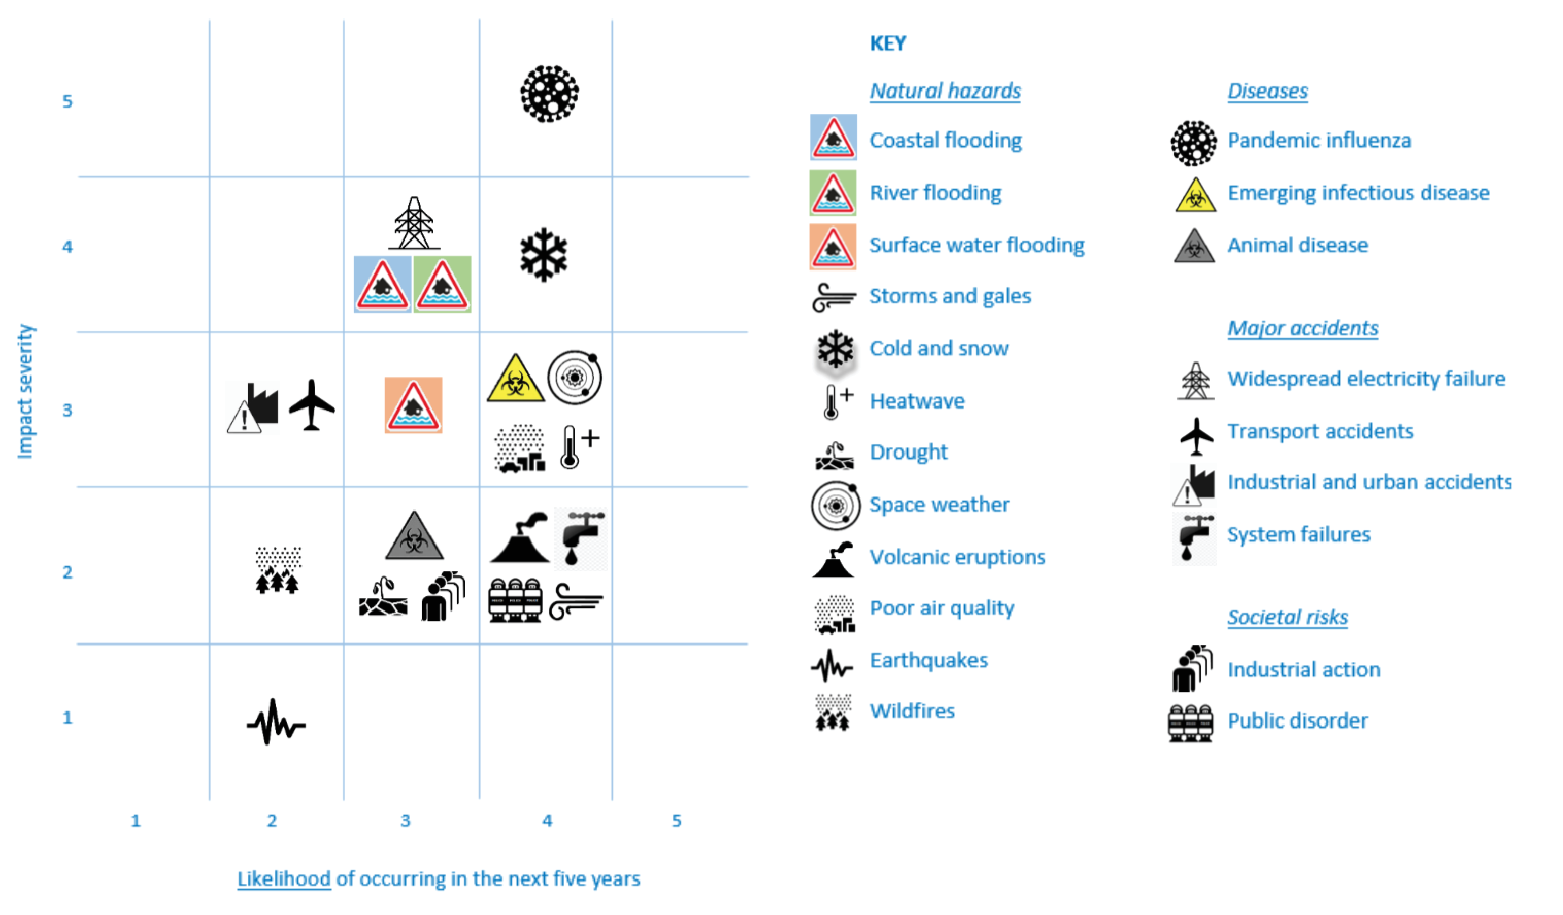
\includegraphics[width=\columnwidth]{UK_risk_register.eps}
	\caption{UK National Risk Register for hazards, diseases, accidents, and societal risks showing space weather as a medium-high risk \citep{cabinet_office_national_2017}}
	\label{fig:UK_Risk_reg}
\end{figure}

An alarming aspect of Figure~\ref{fig:UK_Risk_reg} is that the likelihood of space weather events occurring in 5 years from 2017 was rated the same as pandemic influenza. Finishing this Ph.D. during a global pandemic highlights the importance of taking this risk register very seriously. We should learn from the global response to the COVID-19 pandemic and ensure that the world has a resolute plan to deal with the occurrence of a severe space weather event.

There are many ways that technological systems are impacted by space weather both on or above ground and Figure \ref{fig:space_weather_impacts} displays many of the key impacts that we know of \citep{beggan_ground_2018}. 


\begin{figure}[ht!]
	\centering
	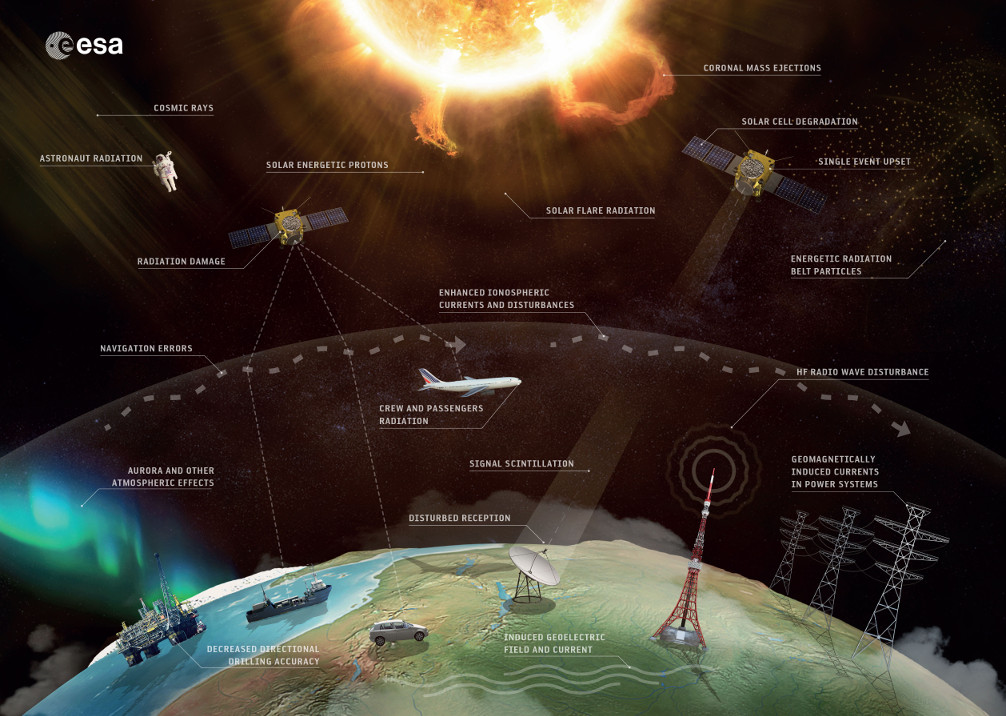
\includegraphics[width=\columnwidth]{Space_weather_effects_rescaled.jpg}
	\caption{The sources and effects of space weather. Impacts are shown including loss of telecommunications and GNSS, increased radiation levels, and ground induced currents (ESA/Science Office, \href{http://www.esa.int/spaceinimages/ESA_Multimedia/Copyright_Notice_Images}{CC BY-SA 3.0 IGO})}
	\label{fig:space_weather_impacts}
\end{figure}

As far back as October 1841 it was reported that a solar storm was responsible for railway disruptions around Exeter, due to magnetic disturbances making it impossible to ascertain whether the onward line was clear, leading to delays \citep{nature_observations_1871}. 

It is possible for space weather events to induce geomagnetic storms that can cause damaging \glspl{gic} within large power grids, causing them to fail. Two such famous cases of \gls{gic} grid failures were in Quebec, Canada in 1989 which resulted in the failure of the Quebec-Hydro grid for 9 hours, and the city-wide black-out in Malm{\"o}, Sweden, during the Halloween storm in 2003 \citep{viljanen_european_2011, beggan_ground_2018}.

It was documented that in May 1967 the U.S. Air Force was close to engaging in conflict with its enemies -- during those politically tense times -- due to the misinterpretation of the effects of space weather \citep{knipp_may_2016}. \glspl{srb}-induced radio frequency interference was initially interpreted as surveillance jamming, an act of war. Fortunately, the U.S. had begun monitoring the space environment and were able determine that space weather was really the cause of the disruption, hence avoiding further conflict \citep{knipp_may_2016}. Furthermore, in more modern times, scintillation effects induced in the ionosphere affect \gls{gnss} communications which has a large societal effect due to our reliance on \gls{gnss} \citep{cannon_extreme_2013} as shown in Figure \ref{fig:space_weather_impacts}.

Solar storms are also responsible for creating sudden increases in ionising radiation which at typical flight altitudes can lead to the risk of malfunctions in aircraft microelectronic systems and unquantified radiation doses to passengers and crew \citep{cannon_extreme_2013}. In orbit these conditions threaten the operation of satellites and the safety of manned space endeavours which is of particular concern with the current ambitions to return to the Moon and venture to Mars. 

There are even concerns that major storms could cause radiation increases at the Earth's surface, \glspl{gle}, which may cause malfunctions in microelectronics that are likely to be of increasing concern in the design of safety-critical systems \citep{cannon_extreme_2013}. 

Finally, a cost analysis estimated a present-day total U.S. economic cost for a super storm on the scale of the 1859 Carrington event \citep{homeier_solar_2013}. The cost estimated is heavily dependent on the duration of outages, the damages caused, and the availability of spare parts for repair; however they estimated the impact on the U.S. economy to be at around \$0.6--2.6 trillion \citep{homeier_solar_2013}. These figures show the large scale impact that space weather can have on the economy and that mitigation techniques to reduce this cost are of imperative necessity.

Due to the many ways that space weather can impact civilisation, and that it is predicted that there is a significant probably of the re-occurrence of large solar storms, it is easy to understand why space weather forecasting is becoming increasingly more necessary as a mitigation technique. 

The U.S. \gls{noaa} is the leading global space weather forecasting agency. The \gls{noaa} \gls{swpc} gathers data in real-time to describe the conditions of the Sun, heliosphere, magnetosphere, and ionosphere to understand the environment within the heliosphere and on Earth. With these data, the \gls{swpc} produces forecasts, warnings, and alerts available to inform anyone concerned and affected by space weather \citep{noaa_noaa_2018}. 

Following the addition of space weather to the UK risk register, the UK \gls{moswoc} opened in 2014 \citep{bis_space_2015}. \gls{moswoc} is mandated to produce daily space weather forecasts and is therefore developing a forecasting infrastructure using ground-based and satellite instrumentation to monitor space weather events. In addition scientific research at \gls{moswoc} is carried out to better understand the physical processes involved in space weather phenomena to improve forecasting accuracy and lead-times; current forecasting enables prediction of \glspl{cme} impacting Earth to within only plus or minus six hours at best \citep{metoffice_space_2013}.

Forecasting and prediction is one aspect of the response to severe space weather events. We must also learn from the global response to the COVID-19 pandemic and ensure that upon the occurrence of a severe space weather event, suitable preplanning has been performed and a sufficient contingent action is planned.





\glsresetall 
{}
%%%%%%%%%%%%%%%%%%%%%%%%%%%%%%%%%%%%%%%%%%%%%%%%%%%%%%%%%%%%%%%%%%%%%%%%
%%%%%%%%%%%%%%%%%%%%%%%%%%%%%%%%%%%%%%%%%%%%%%%%%%%%%%%%%%%%%%%%%%%%%%%%
%%%%%%%%%%%%%%%%%%%%%%%%%%%%%%%%%%%%%%%%%%%%%%%%%%%%%%%%%%%%%%%%%%%%%%%%
\section{Cosmic Rays}\label{sec:intro_CRs}

\subsection{Background}
%The first accounts of measurement of \glspl{cr} date back to the 18th century, when scientists reported observations of spontaneous ionisation; however generally they were initially disregarded as they were believed to be due to imperfect experimental conditions \citep{montanus_observability_2017}. It was not until the late 19th and early 20th century that the nature of this spontaneous ionisation was understood to be caused by \glspl{cr}. 

\glspl{cr} are charged particles and atomic nuclei with energies spanning from 1~keV up to around $10^{21}$~eV, that encroach upon the Earth from all directions \citep{giacalone_energetic_2010}. It is understood that \glspl{cr} are composed of $\sim99\%$ of atomic nuclei and $\sim1\%$ electrons \citep{gaisser_cosmic_2016}; of the atomic nuclei $\sim87\%$ are protons, $\sim12\%$ are $\alpha$-particles, and a smaller contribution of $\sim1\%$ are heavier nuclei of around $\sim1\%$ \citep{grupen_astroparticle_2005, dunai_cosmic_2010, particle_data_group_review_2020}. \glspl{cr} mainly originate from outside the solar system, known as \glspl{gcr} \citep{particle_data_group_review_2020}. These \glspl{gcr} mostly come from within the Milky Way, although they are also expected to emanate from extra-galactic sources, in particular for \glspl{cr} with energies above $10^{18}$~eV \citep{aab_observation_2017}. Incoming low-energy \glspl{cr} ($\lesssim1$~GeV/nucleon) are modulated by the solar wind, which decelerates \glspl{gcr} and can even forbid lower-energy \glspl{gcr} from the inner solar system \citep{grupen_astroparticle_2005}. Consequently, there exists a strong anti-correlation between solar activity and the \glspl{gcr} flux \citep{particle_data_group_review_2020}.

Cosmic rays produced within the heliosphere are mostly of solar origin, known as \glspl{scr} or \glspl{sep}. These \glspl{scr} are generally of a lower energy than \glspl{gcr} and may be accelerated in the solar wind, by interplanetary shocks, or in solar eruptions (e.g. solar flares) \citep{giacalone_energetic_2010}. \glspl{scr} have typical energies on the order of magnitude of $\sim10^{1}$~keV--$1$~GeV \citep{chilingarian_galactic_2003, bruno_solar_2018}. Therefore \glspl{pcr} associated with space weather events are generally of much lower energy than the background of \glspl{gcr}.

The intensity spectrum of \glspl{pcr} in the energy range from $10^9$~eV to $\sim10^{14}$~eV is given approximately by:

\begin{equation}
\label{eq:CR_flux}
I_N(E) = \frac{dN}{dE} \approx 1.8 \, \mathsf{x} \, 10^4 (E/1 \, \mathrm{GeV})^{-\alpha} \frac{\mathrm{nucleons}}{{\mathrm{m^2 \, s  \, sr \, GeV}}} \, ,
\end{equation}
%
where $E$ is the energy per nucleon (including rest mass energy) in GeV and $\alpha=2.7$ is the differential spectral index of the cosmic-ray flux \citep{particle_data_group_review_2020}. 

Figure~\ref{fig:CR_spec} shows a graphical representation of the \gls{cr} energy spectrum described by equation~(\ref{eq:CR_flux}). It shows the flux for a number of \gls{cr} species, over the energy range $10^{-1}$--$10^{6}$~GeV/nucleus, measured by several different experiments.

\begin{figure}[ht!]
	\centering
	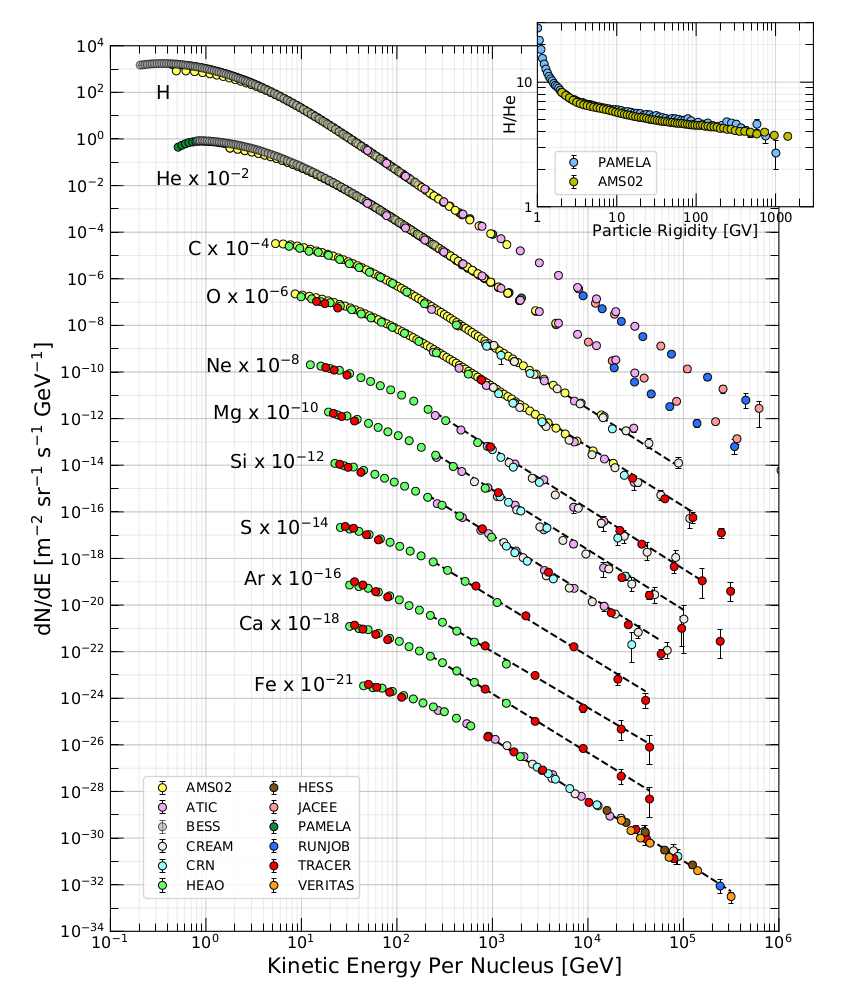
\includegraphics[width=0.8\columnwidth]{CR_spectrum.png}
	\caption{ Cosmic ray differential energy spectrum using data measured by several experiments. The inset shows the H/He ratio at constant rigidity \citep{particle_data_group_review_2020} }
	\label{fig:CR_spec}
\end{figure}

Beyond the x-axis range in Figure~\ref{fig:CR_spec}, the spectrum `knee' occurs (i.e. in the range $\sim10^{15}$--$10^{16}$~eV) where the spectral index is thought to increase to $\sim3$ \citep{particle_data_group_review_2020}. At even higher energies, in the region of the spectrum `ankle' ($\sim10^{18.5}$~eV) the spectral index reduces and the spectrum becomes less steep. This is in the regime of \glspl{uhecr} and the interaction between \glspl{gcr} and photons of the \gls{cmb} sets an upper limit on their energy, the \gls{gzk} limit \citep{particle_data_group_review_2020}. The \gls{gzk} limit implies that \glspl{cr} with energies exceeding $\sim5\times10^{19}$~eV must have originated from distances within a horizon of $\sim50$~Mpc, as otherwise their energy would have been reduced by the \gls{gzk} effect \citep{particle_data_group_review_2020}. 


Propagation of \glspl{cr} through magnetic fields depends on their gyroradius or Larmor radius \citep{particle_data_group_review_2020}. Therefore a common description of \glspl{cr} uses a property called the {\textit{magnetic rigidity}} which is defined by:

\begin{equation}
\label{eq:rigidity}
R = r_L \, B \, c = \frac{p \, c}{Z \, e}
\end{equation}
%
where $r_L$ is the Larmor radius, $B$ is the magnetic field strength, $c$ is the speed of light, $p$ is the particle's momentum, $Z$ is the atomic number, and $e$ is the electron charge. The magnetic rigidity has units of Volts (V), or usually due to a large magnitude, Gigavolts (GV). The rigidity is used to describe \glspl{cr} as particles with different charges and masses have the same dynamics in a magnetic field if they have the same rigidity \citep{particle_data_group_review_2020}.



\subsection{Cosmic Rays in the Atmosphere}
\label{sec:air_shower}

\glspl{cr} in the interstellar medium traverse a very low-density medium, but experience a much denser environment when they reach the atmosphere. The typical nucleon mean free path (measured in units of $\mathrm{g}\,\mathrm{cm}^{-2}$) of protons in the atmosphere is $\sim90~\mathrm{g}\,\mathrm{cm}^{-2}$, which means the first interactions of \glspl{cr} occur in the upper layers of the atmosphere, at a height of $\sim15$--$20$~km \citep{grupen_astroparticle_2005}. %scale height used to calculate this, i.e. if X = X_0 exp(-h/H), where X is the atmospheric depth (g/cm2), X_0 is sea level atmospheric depth (1030 g/cm2), H is scale height (~8.5km), then rearranging finds h ~ 20km.

The \glspl{pcr} will predominantly interact with the atmospheric nuclei via strong interactions \citep{grupen_astroparticle_2005}. When \glspl{pcr} interact with atmospheric nuclei, the interaction leads to the production of a cascade of secondary particles. The secondary particles can also undergo interaction or decay, producing tertiary particles, and the process continues until all the particles' energy is insufficient to create new particles. If a concentrated, large number of secondary particles reach ground-level, the cascade of particles is called an \gls{as}, or an \gls{eas} for extremely high numbers of secondary particles, which can have a footprint area of several~km$^2$. The \gls{as} is often described as being a cone, with the base being the shower front and the apex being the primary \gls{cr}.

Hadronic cascade components (or the ``hard component" of \glspl{as}) are produced by \gls{cr} protons and nuclei interacting with atmospheric nuclei. This process typically produces lower energy protons, neutrons, pions, and kaons. In this thesis we are mostly interested in the muonic air shower development (see Section~\ref{sec:intro_HiSPARC}), so here we will focus on the development of the mesons in the \glspl{as}, as they predominantly produce muons. In Table~\ref{tab:meson_decay}, the most likely modes of decay for air shower mesons are shown with the branching ratio for each mode. In addition, the table also shows the most likely decay modes of muons.


\begin{table}[ht!]
	\begin{center}
		\caption{ Most prominent decay modes of the mesonic components of CR air showers and of muons. Note: $K^-$ modes are charge conjugates of the decay modes below \citep{particle_data_group_review_2020}}
		\label{tab:meson_decay}
		\begin{tabular}{lc}
			\hline
			Decay mode & Branching ratio  \\
			\hline
			{$ \pi^{+} \, \rightarrow \, \mu^{+} \, + \, \nu_{\mu} $}	 &  $99.98770 \pm 0.00004 \%$ \\
			{$ \pi^{-} \, \rightarrow \, \mu^{-} \, + \, \overline{\nu_{\mu}} $}  &  $99.98770 \pm 0.00004 \% $ \\
			{$ \pi^{0} \, \rightarrow \, \gamma \, + \, \gamma $} &  $98.823 \pm 0.034 \% $ \\
			{$ \pi^{0} \, \rightarrow \, e^+ \, + \, e^-  \, + \, \gamma $} &  $1.174 \pm 0.035 \% $ \\
			{}  & {} \\
			{$K^+ \, \rightarrow \, \mu^{+} \, + \, \nu_{\mu}$}  &  $63.56 \pm 0.11 \% $ \\
			{$K^+ \, \rightarrow \, \pi^{+} \, + \pi^{0} $}  &  $20.67 \pm 0.08 \% $ \\
			{$K^+ \, \rightarrow \, \pi^{+} \, + \pi^{+} \, + \pi^{-}$}  &  $5.583 \pm 0.024 \% $ \\
			{$K^+ \, \rightarrow \, \pi^{0} \, + e^{+} \, + \nu_{e}$}  & $5.07 \pm 0.04 \% $ \\ 		 		 		 		
			{$K^+ \, \rightarrow \, \pi^{0} \, + \mu^{+} \, + \nu_{\mu}$}  &  $3.352 \pm 0.033 \% $\\ 		 		 		 		
			{$K^+ \, \rightarrow \, \pi^{+} \, + \pi^{0} \, + \pi^{0}$}  &  $1.760 \pm 0.023 \% $\\
			{}  & {} \\
			{$ \mu^{+} \, \rightarrow \, e^{+} \, + \, \nu_e \, + \, \overline{\nu_{\mu}} $}  &  $\sim 100\%$\\	
			{$ \mu^{-} \, \rightarrow \, e^{-} \, + \, \overline{\nu_e} \, + \, \nu_{\mu} $}  &  $\sim 100\%$\\	
			\hline
		\end{tabular}
	\end{center}
\end{table}


Due to the short lifetimes of pions and kaons, $\sim26$~ns and $\sim12$~ns, respectively \citep{particle_data_group_review_2020}, and depending on energy, they decay during their journey to ground-level. It is shown in Table~\ref{tab:meson_decay} that the most probable decay modes involve the production of muons. Muons are the most abundant charged particles at ground level \citep{particle_data_group_review_2020}. Most muons are produced high in the atmosphere ($\sim15$~km) and lose about 2~GeV to ionization before reaching the ground and the mean energy of muons at the ground is $\sim4$~GeV \citep{particle_data_group_review_2020}.

%; hence when produced at low enough altitudes allowing enough time for these muons to reach ground, there is a large muon contingent at the ground level. At sea level the average kinetic energy of muons is approximately 4 GeV \citep{bartels_hisparc_2012}.

In addition to the hadronic component of an air shower, electron and photon constituents of cascades are called the electromagnetic component (or ``soft component"). These are typically initiated by electrons and photons under the processes of Bremsstrahlung \citep{grupen_astroparticle_2005},

\begin{equation}
\label{eq:bremss}
e \, \rightarrow \, e \, + \, \gamma \, ,
\end{equation}
%
or pair production \citep{grupen_astroparticle_2005},
%
\begin{equation}
\label{eq:pair_prod}
\gamma \, \rightarrow \, e^- \, + \, e^+ \, .
\end{equation}

Ionisation losses mean that electrons and positrons lose energy rapidly until they either annihilate or recombine with nuclei, and photons lose their energy by being either absorbed in scattering and/or the photoelectric effect. Therefore most of the electrons, positrons,
and photons observed at ground level are produced from the decaying hadronic \gls{as} component and muon decay is the dominant source of low-energy electrons at ground level \citep{particle_data_group_review_2020}.

Finally, there is a minimum rigidity cut-off which implies that the energy of any \gls{pcr} must exceed a minimum energy to be able to initiate an \gls{as} or particle cascade and be measured at ground-level. This limit is dependent on the depth of the atmosphere above the detector, but is greatest at sea-level and decreases with increasing altitude. The minimum energy to be measured at sea-level is approx. $430$~MeV/nucleon \citep{dorman_theory_2004, dorman_experimental_2004, poluianov_gle_2017}.



\subsection{Cosmic Ray Detectors}

To observe \glspl{cr} there are many types of usable detectors, both ground-based and space-based \citep{schrijver_heliophysics_2010}; in this thesis we are mostly concerned with ground-based detectors of the \gls{as} hadronic component. The most common type of ground-based \gls{cr} detectors are \glspl{nm} and \glspl{md} which indirectly measure \gls{cr} particles through the secondary particles produced in \gls{cr} cascades. These two types of detector probe different energy ranges; \glspl{nm} generally observe \glspl{pcr} with energies $\sim$1--10~GeV and above, while \glspl{md} typically observe higher energy \glspl{pcr} with energies on the order of $\gtrsim10$~GeV \citep{kuwabara_real-time_2006, rockenbach_global_2014}.

\subsubsection*{Neutron Monitors}
The neutron monitor, invented by \cite{simpson_latitude_1948}, has been extensively used for \gls{cr} observations of the space environment \citep{clem_neutron_2000}. The \gls{nm} is an example of an ionisation detector whereby energetic neutrons encounter a nucleus within a gas, producing charged, secondary particles which in turn ionise the surrounding gas \citep{gloeckler_-situ_2010}.

The original ``IGY" \gls{nm} design made use of a paraffin reflector to trap slow neutrons within the detector, a producer material (typically lead) which multiplied the number of slow neutrons registered by the detector in order to amplify the signal, a moderator to further slow neutrons, and cylindrical proportional counters utilising BF\textsubscript{3} gas \citep{simpson_latitude_1948, simpson_cosmic_1953}. A schematic diagram of the detector is shown in Figure~\ref{fig:NMIGY}. %The proportional counter is essentially a gas-filled chamber with two electrodes; a potential difference between the electrodes attracts the ionised gas collecting positive and negative charge which results in charge appearing across a coupling capacitor \citep{schrijver_heliophysics_2010}. Following the discharge of the capacitor, the signal is then amplified and recorded through the back-end electronics \citep{simpson_latitude_1948, simpson_cosmic_1953}.

\begin{figure}[ht!]
	\centering
	\subfloat[Standard IGY]{{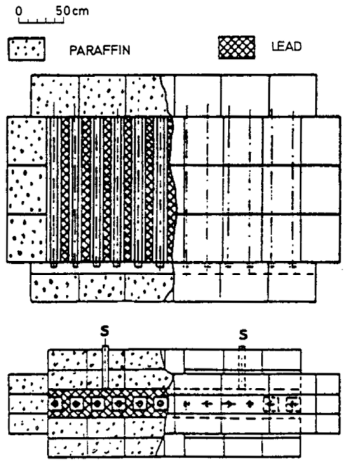
\includegraphics[width=0.36\columnwidth]{NM_IGY_rescaled.png} } \label{fig:NMIGY}}%
	\qquad
	\subfloat[6-tube NM64]{{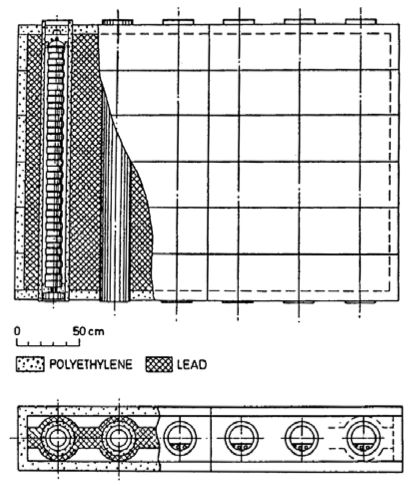
\includegraphics[width=0.36\columnwidth]{NM_64_rescaled.png} } \label{fig:NM64}}%
	\caption{Schematic diagrams of two NM configurations: (a) the original Simpson's 12-tube IGY NM is shown where the paraffin reflector is represented by the outer dotted blocks; the lead producer is represented by the cross-hatched section; the paraffin moderator is represented by the inner dotted blocks; finally the gas-filled proportional counters are denoted by the black circles/tubes. (b) the modern NM64 is shown on the right in its 6-tube configuration where the polyethylene reflector is represented by the outer dotted section; the lead producer is represented by the cross-hatched area; within the producer is a cylindrical polyethylene moderator denoted by the dotted ring; finally in the centre of each tube is a gas-filled proportional counter. In each figure the top schematic is a top-down drawing and the bottom is an end-on drawing. Taken from \citet{kang_characteristics_2012}.}
	\label{fig:NM}
\end{figure}

An improved ``NM64" \gls{nm} design is now the preferred detector type, which makes use of a polyethylene reflector, lead producer, polyethylene moderator, and \textsuperscript{10}BF\textsubscript{3} or \textsuperscript{3}He gas-filled cylindrical proportional counters \citep{kang_characteristics_2012}. A schematic diagram of the detector is shown in Figure~\ref{fig:NM64}. The new design provided an improvement over the IGY design by a factor of about 3.3 in the count rate per unit area of producer \citep{stoker_neutron_2000}; the choice of \textsuperscript{10}BF\textsubscript{3} gas or \textsuperscript{3}He gas does not significantly affect the detector performance \citep{kang_characteristics_2012}.



\subsubsection*{Muon Detectors}

Muon detectors are an example of a scintillation detector, whereby light emitted by atoms excited in a medium is collected and converted into an electrical signal. The scintillation medium can be solid, liquid, or gas; however solid scintillation detectors are attractive as they have a higher electron density \citep{gloeckler_-situ_2010}.

A general design of a \gls{md} is shown in Figure~\ref{fig:MD}. When an energetic particle passes through a scintillator material, some of the particle's energy is lost in ionising the scintillator material and the scintillator material releases photons. The light pipe directs the photons towards a \gls{pmt} where a cascade of electrons are produced and the resulting electrical signal is amplified and recorded through the back-end electronics.

\begin{figure}[ht]
	\centering
	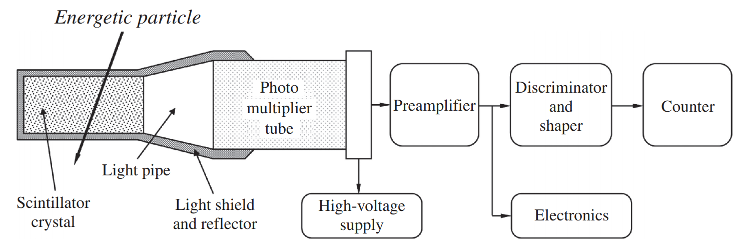
\includegraphics[width=0.7\columnwidth]{scintillator_rescaled.png}
	\caption{Schematic design of a typical scintillation muon detector with back-end electronics \citep{gloeckler_-situ_2010}}
	\label{fig:MD}
\end{figure}

Desirable properties of scintillator materials are a high conversion efficiency, transparency to the light that they emit, short fluorescent decay times, and spectral distributions suitable for photosensitive devices \citep{gloeckler_-situ_2010}. 

A range of different material types are used in scintillator detectors however the most common scintillator materials for \glspl{md} are organic scintillators consisting of aromatic hydrocarbons (the fluors) in a solid plastic solvent (the base) \citep{gloeckler_-situ_2010, fokkema_hisparc_2012}. Energetic particles traversing the scintillator excite the base rather than the fluor due to the low fluor density. The plastic base however has a low yield and is not transparent to its own scintillation light; thus the fluor is added to therefore increase the yield of this popular type of scintillator \citep{fokkema_hisparc_2012}.





\subsection{Cosmic Ray Observations of Solar Activity and Space Weather}

It has long been established that there exists an anti-correlation between \gls{gcr} intensity and the level of solar activity, over the $\sim11$-year period \citep{forbush_cosmic-ray_1958, parker_passage_1965, usoskin_correlative_1998, van_allen_modulation_2000}. We also see the 22-year Hale cycle manifesting in the \gls{gcr} intensity, as interchanging peaked and flat-topped cycles of \gls{gcr} intensity due to combination of solar activity and \gls{cr} transport processes \citep{aslam_solar_2012, thomas_22-year_2014}, as seen in Figure~\ref{fig:gcr_plot}. The effects of solar activity on \glspl{cr} observations are discussed in more details in the introduction to Chapter~\ref{chap:GCR_SSN_24}.
%The positively charged cosmic rays drift in from the heliospheric polar regions when the Sun’s north polar field is directed outward (positive). When the Sun’s north polar field is directed inward (negative) the positively charged cosmic rays drift inward along the heliospheric current sheet where they are scattered by corrugations in the current sheet and by magnetic clouds from CMEs. The negatively charged cosmic rays (electrons) drift inward from directions (polar or equatorial) opposite to the positively charged cosmic rays that are detected by neutron monitors.

\begin{figure}[ht!]
	\centering
	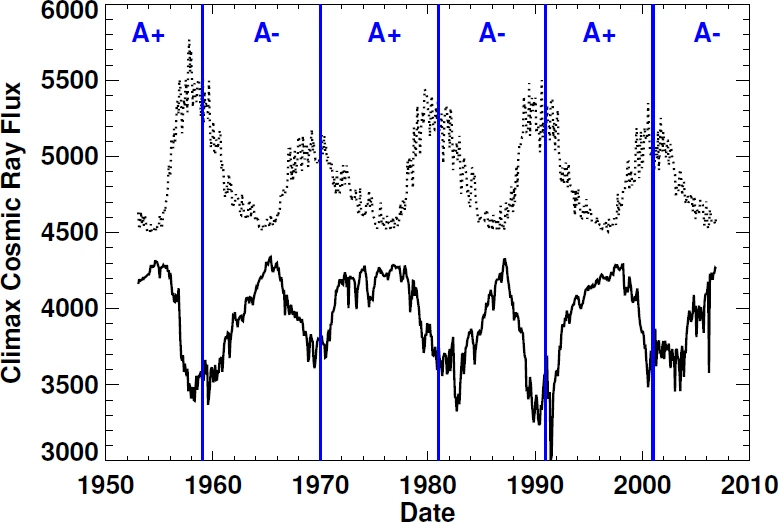
\includegraphics[width=0.95\columnwidth]{gcr.png}
	\caption{Cosmic ray flux measured at the Climax NM (solid line) and rescaled SSN (dotted line) taken from \citet{hathaway_solar_2015}. The vertical lines denote changes in the Sun's global magnetic field polarity, where: A$+$ indicates positive polarity at the North Pole; A$-$ indicates negative polarity at the North Pole.}
	\label{fig:gcr_plot}
\end{figure}

There have been many documented observations of space weather events using \gls{cr} detectors. The most notable types of \gls{cr} space weather effects are \glspl{fd} and \glspl{gle}; here we discuss the properties of each.

\subsubsection*{Forbush Decreases}\label{sec:intro_FDs}

Short-term decreases in the \gls{gcr} flux were first observed by  \citet{forbush_effects_1937} and therefore were later coined as \glspl{fd} or \glspl{fe}. \glspl{fd} are characterised by a sharp decrease in \gls{gcr} intensity over a period of several hours--days, followed by a gradual recovery taking place over several days--a week \citep{cane_coronal_2000, belov_forbush_2008, wawrzynczak_modeling_2010}, as shown in Figure~\ref{fig:FD_plot}.

\begin{figure}[ht!]
	\centering
	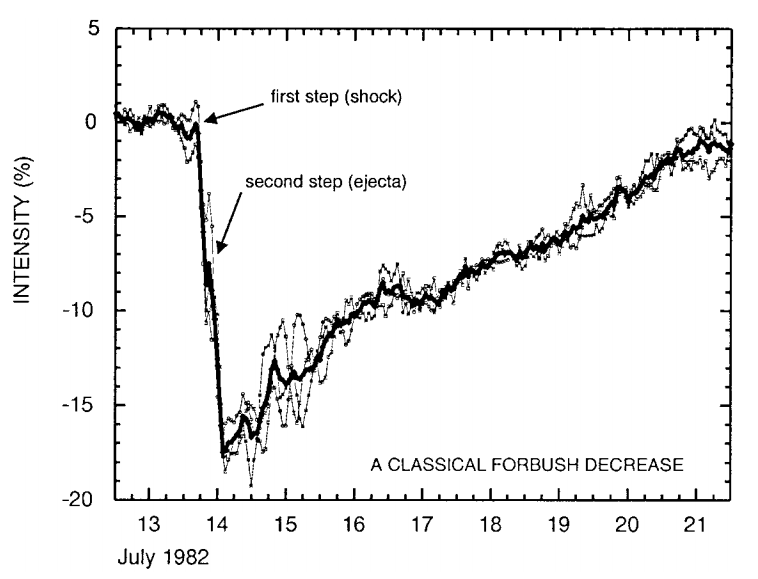
\includegraphics[width=0.75\columnwidth]{FD_plot.png}
	\caption{A two-step Forbush decrease measured at three NM stations, Deep River, Mt.Wellington, Kerguelen, in July 1982 \citep{cane_coronal_2000}. The thicker black line indicates the average of the count rates from the three stations. Arrows show the start of the two decreases caused by the shock and the ICME ejecta.}
	\label{fig:FD_plot}
\end{figure}

There are two \gls{fd} origins: one caused by \glspl{cir} \citep{dumbovic_forbush_2016}, and one caused by \glspl{icme} and the shocks they drive \citep{belov_forbush_2008}. The biggest \glspl{fd} (magnitudes $> 5\%$) are strictly associated with \glspl{icme} \citep{belov_what_2001}. Of the kind caused by \glspl{icme}, the majority are produced by \glspl{icme} with speeds in the range 400--1200~km~s$^{-1}$ \citep{lingri_forbush_2016}; the typical speed of the solar wind is, for slow solar wind, in the range 300--400~km~s$^{-1}$, and for fast solar wind, $\sim 750$~km~s$^{-1}$ \citep{owens_heliospheric_2013}. Previous literature has also shown that the type caused by \glspl{cir} produce recurrent, more symmetric, and lower-amplitude decreases \citep{dumbovic_cosmic_2012}, while the type caused by \glspl{icme} result in the more strongly asymmetric decreases as shown in Figure~\ref{fig:FD_plot} \citep{lockwood_forbush_1971, cane_coronal_2000, dumbovic_cosmic_2012}. In addition the \gls{icme}-driven \glspl{fd} typically result in a two-step \gls{fd}, where the first step of the decrease is due to the passage of the leading shock and the second step is due to the \gls{icme} itself, as shown in Figure~\ref{fig:FD_CME} \citep{cane_coronal_2000}.

\begin{figure}[ht!]
	\centering
	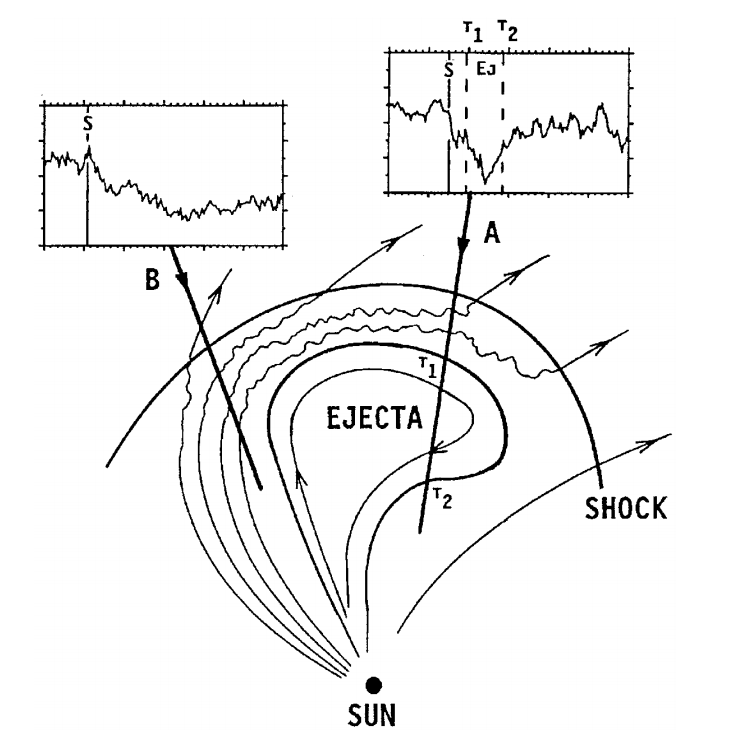
\includegraphics[width=0.75\columnwidth]{FD_CME.png}
	\caption{A schematic diagram of an ICME-driven FD taken from \citet{cane_coronal_2000}. It shows the different cosmic ray responses from two paths, indicated by A and B. A experiences the shock and ejecta, therefore experiencing a two-step FD; B only experiences the shock, therefore experiencing a single decrease. The time of shock passage is indicated by a solid, vertical line marked, S; the start and end times of ejecta passage are indicated by vertical, dashed lines marked T1 and T2, respectively.}
	\label{fig:FD_CME}
\end{figure}

\citet{lockwood_forbush_1971} showed that there is a rigidity dependence on the amplitudes of \glspl{fd}, which is approximately related to $R^{-\gamma}$, where the exponent ranges from $0.4\lesssim\gamma\lesssim1.2$. In addition, \citet{belov_what_2001, belov_coronal_2014} showed the magnitude of the \gls{fd} is proportional to the speed, mass, and width of the \gls{cme}. 


The \gls{feid}\footnote{\url{http://spaceweather.izmiran.ru/eng/dbs.html}} is a record of all the \glspl{fd} observed since the beginning of the \gls{gnmn} \citep{belov_forbush_2008}. The total number of events is $\sim 7630$ during the epoch 1957--2020. Many studies have analysed observations of \glspl{fd} using these data and investigated their features, driving factors, and precursors; for an overview see: \citet{belov_what_2001, usoskin_forbush_2008, wawrzynczak_modeling_2010, rockenbach_global_2014, arunbabu_how_2015}.



\subsubsection*{Ground Level Enhancements}\label{sec:intro_GLEs}

Short-term increases in the \gls{gcr} flux were first observed in the 1940s and early 1950s, but it wasn't until after the largest recorded event, in September 1956, that these increases were defined as \glspl{gle} \citep{cramp_modelling_1996}. \glspl{gle} are the detection of an increased number of the highest-energy portion ($> 500$~MeV, \citet{kuwabara_development_2006}) of \glspl{sep} arriving at Earth along lines of \gls{imf} following a solar eruptive event \citep{mccracken_high-energy_2012, poluianov_revisited_2017}. The \glspl{sep}, which cause \glspl{gle}, can cause serious damage to satellite electronics and are a hazard to air crew and astronauts; hence, the monitoring of these events are of importance for space weather forecasting. \glspl{gle} are characterised by a sharp rise in \gls{cr} intensity over a period of several minutes--hours, followed by a gradual decay taking place over several hours, as shown in Figure~\ref{fig:GLE_plot}. 

\begin{figure}[ht!]
	\centering
	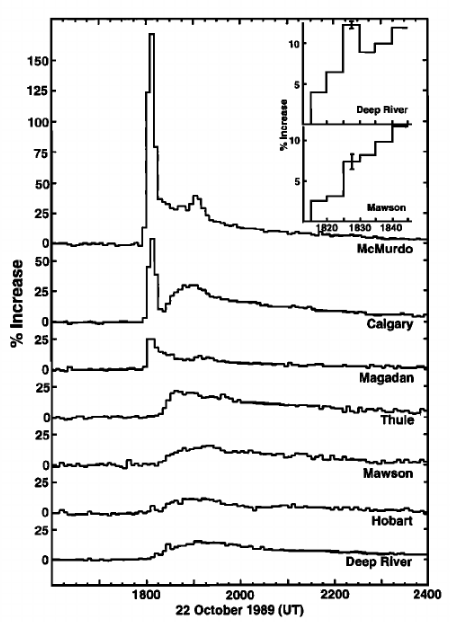
\includegraphics[width=0.75\columnwidth]{GLE_plot.png}
	\caption{A GLE measured at nine NM stations in October 1989, taken from \citet{cramp_j._l._october_1997}.}
	\label{fig:GLE_plot}
\end{figure}


\glspl{gle} result from energetic solar eruptions such as flares and \glspl{cme} \citep{mccracken_high-energy_2012}. The total number of \glspl{gle} observed to-date is low: there have been only 72. The \gls{gle} database\footnote{\url{https://gle.oulu.fi}} is a record of events, starting from \gls{gle} 5 (February 1956), since the beginning of the \gls{gnmn} \citep{usoskin_database_2016}. Many studies have discussed the observations of \glspl{gle}, investigating their features as well as the spectra and anisotropy of \glspl{pcr} that produce the \glspl{gle}; for an overview see: \citet{,shea_possible_1982, cramp_modelling_1996, belov_ground_2010, mccracken_high-energy_2012, strauss_pulse_2017,  mishev_first_2018}. \citet{strauss_pulse_2017} analysed the shapes of fourteen \glspl{gle} and showed the existence of a linear dependence between the rise and decay times which they empirically determined to be $\tau_d\approx3.5\tau_r$.

The solar magnetic field is `frozen' into the solar wind plasma. As the Sun rotates, so do the \gls{imf} lines which forms an Archimedean spiral, the Parker spiral \citep{parker_dynamics_1958, parker_spiral_1976}. A curved field line connecting the Sun to the Earth stems from the western limb of the Sun, at a longitude of about $60^{\circ}$, which is known as the `garden hose' field line (see Fig.~\ref{fig:garden_hose}) \citep{duldig_ground_1993, hathaway_solar_2015}. Charged particles follow magnetic field lines and therefore \glspl{sep} that are accelerated in flares located near to the solar end of the `garden hose' field line usually arrive at Earth rapidly and have very sharp onsets \citep{duldig_ground_1993, andriopoulou_intense_2011}. This causes a strong anisotropy in the arrival directions of the early \glspl{sep} inducing \glspl{gle}, as shown in Figure~\ref{fig:GLE_plot}. The McMurdo, Calgary, and Magaden \gls{nm} stations observed an earlier \gls{gle} onset, with a high magnitude, than the other stations \citep{duldig_ground_1993, cramp_j._l._october_1997}. Conversely, \glspl{gle} associated with flares far from the `garden hose' field line are usually delayed in their arrival at Earth, due to having to cross magnetic field lines, and have more gradual increases to maximum intensity \citep{duldig_ground_1993}. Very few \glspl{gle} have originated far away from the base of the `garden hose' at the solar surface \citep{duldig_ground_1993, andriopoulou_intense_2011}.

\begin{figure}[ht!]
	\centering
	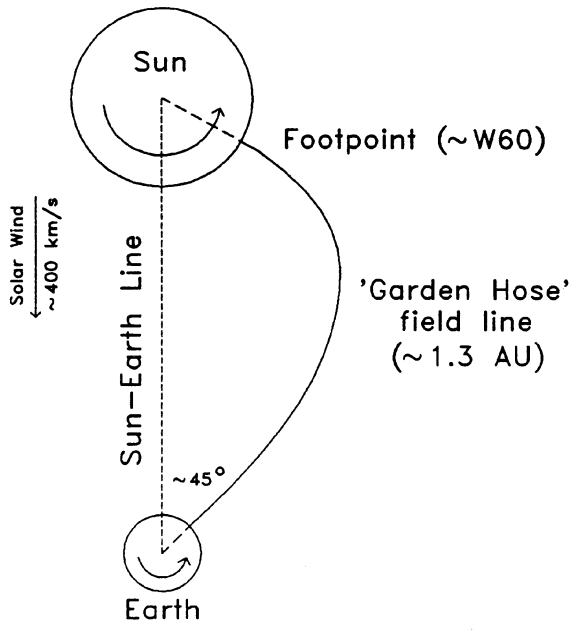
\includegraphics[width=0.75\columnwidth]{garden_hose.png}
	\caption{A schematic diagram of the `garden hose' field line taken from \cite{duldig_ground_1993}.}
	\label{fig:garden_hose}
\end{figure}

The accepted definition of a \gls{gle} since the 1970s has been \citep{poluianov_gle_2017}: 

\begin{quote}
	\textit{a GLE event is registered when there are near-time coincident and statistically significant enhancements of the count rates of at least two differently located NMs.}
\end{quote}

However, recently a newer \gls{gle} definition has been adopted due to the increase in the number of \gls{nm} stations that are more sensitive to lower energy \glspl{cr} due to their high latitudes (i.e. in near-polar regions) or higher altitudes. It is a concern that these new \gls{nm} stations will classify many more \glspl{gle} than their near-sea-level counterparts, thus affecting the homogeneity of the current list of \glspl{gle} \citep{poluianov_gle_2017}. Therefore the new \gls{gle} definition is as follows \citep{poluianov_gle_2017}: 

\begin{quote}
	\textit{a GLE event is registered when there are near-time coincident and statistically significant enhancements of the count rates of at least two differently located neutron monitors, including at least one neutron monitor near sea-level and a corresponding enhancement in the proton flux measured by a space-borne instrument(s).}
\end{quote}

The new definition also invoked the introduction of a sub-\gls{gle} class, defined as \citep{poluianov_gle_2017}:

\begin{quote}
	\textit{a sub-GLE event is registered when there are near-time coincident and statistically significant enhancements of the count rates of at least two differently located high-elevation neutron monitors and a corresponding enhancement in the proton flux measured by a space-borne instrument(s), but no statistically significant enhancement in the count rates of neutron monitors near sea level.}
\end{quote}


Finally, a \gls{gle} real-time alarm system was developed by \citet{kuwabara_real-time_2006, kuwabara_development_2006}, using data from \glspl{nm} and \glspl{md}, which has been shown to provide the earliest alert for the onset of \gls{sep}-driven space weather events. They showed their alerts provide a warning up to an hour earlier than the storm onset. Furthermore, they also show that through utilising the \gls{gnmn}, monitoring precursory anisotropy, they can also issue warnings several hours ahead of near-Earth, in-situ satellite observations. They state that using both \glspl{nm} and \glspl{md} provides a dual energy range for observations, providing a more effective system.


\glsresetall 
{}
%%%%%%%%%%%%%%%%%%%%%%%%%%%%%%%%%%%%%%%%%%%%%%%%%%%%%%%%%%%%%%%%%%%%%%%%
%%%%%%%%%%%%%%%%%%%%%%%%%%%%%%%%%%%%%%%%%%%%%%%%%%%%%%%%%%%%%%%%%%%%%%%%
%%%%%%%%%%%%%%%%%%%%%%%%%%%%%%%%%%%%%%%%%%%%%%%%%%%%%%%%%%%%%%%%%%%%%%%%
\section{The HiSPARC Experiment}\label{sec:intro_HiSPARC}

%%%%%%%%%%%%%%%%%%%%%%%%%%%%%%%%%%%%%%%%%%%%%%%%%%%%%%%%%%%%%%%%%%%%%%%%
\subsection{Background}

The \gls{hisparc} is a scientific outreach project that was initiated in the Netherlands in 2002 \citep{bartels_hisparc_2012}. The \gls{hisparc} experiment has two main goals: the study of \gls{uhecr} for astroparticle physics research, and to serve as a resource to expose high school students to scientific research \citep{bartels_hisparc_2012}.

\gls{hisparc} is a global network of muon detectors spread across the Netherlands, Denmark, the UK, and Namibia. There are $\sim140$ stations in the \gls{hisparc} network \citep{van_dam_hisparc_2020} which have been uploading data for varying durations since 2005. The detection philosophy of \gls{hisparc} is to sample the footprints of \glspl{eas} using coincident triggers between scintillation detectors. The detectors at each station record muon counts and may be used for many scientific experiments, such as: reconstruction of the direction of a cosmic ray induced air shower, reconstruction of the energy of the air shower's primary particle, investigation between the atmospheric conditions and the number of cosmic rays observed, etc. A comprehensive review of the \gls{hisparc} experiment is provided by \citet{fokkema_hisparc_2012} and \citet{van_dam_hisparc_2020}.

The \gls{hisparc} network has predominantly been used to study \glspl{uhecr}, i.e. \glspl{pcr} with energies in excess of $\sim10^{14}$~eV. However, \citet{van_dam_probing_2020} used the \gls{hisparc} data to derive the \gls{cr} flux at sea level for \glspl{pcr} with energies between $10^{12}$--$10^{16}$~eV. Furthermore, \citet{fan_analysis_2018} provided a study into the anti-correlation between atmospheric pressure and the \gls{hisparc} data, as well as claiming to demonstrate the correlation between the daily-average of \gls{cr} events and characteristic solar activity parameters.



%%%%%%%%%%%%%%%%%%%%%%%%%%%%%%%%%%%%%%%%%%%%%%%%%%%%%%%%%%%%%%%%%%%%%
\subsection{HiSPARC Detector and Station Configuration}

As \gls{hisparc} was set up as an outreach programme for high schools, this impacted detector design \citet{fokkema_hisparc_2012, van_dam_hisparc_2020}. Resources are limited in schools and the detectors are usually financed by the participating high schools, colleges, and universities. In addition, students (accompanied by their teachers and local node support staff) are responsible for assembly and installation of their detectors, which are typically installed on the roofs of schools. Due to this, the detectors needed to be cheap, robust, and easily maintainable, therefore the scintillation detector was selected for the \gls{hisparc} network.

Scintillators consist of materials that emit light when charged particles pass through them with sufficient energy to ionise the scintillator material. The total light produced is proportional to the number of charged particles, and can be collected by a \gls{pmt}. Each \gls{hisparc} detector utilises a plastic scintillator of dimensions $1000$~mm~$\times~500$~mm~$\times~20$~mm, providing a detection area of 0.5~$\mathrm{m}^2$. A vertically incident \gls{mip} has a most probable energy loss in 2~cm of the scintillation material of 3.51~MeV ($\equiv 1$ \gls{mip}) \citep{van_dam_hisparc_2020}.

The scintillator is glued to a triangular/`fish-tailed' light-guide (dimensions, base: 500~mm; top: 25~mm; height: 675~mm), and a light-guide adapter provides the optical interface between the square end of the light-guide and the cylindrical aperture of the \gls{pmt}. The configuration of a single \gls{hisparc} detector is shown in Figure~\ref{fig:HS_scintillator}. 

\begin{figure}[ht!]
	\centering
	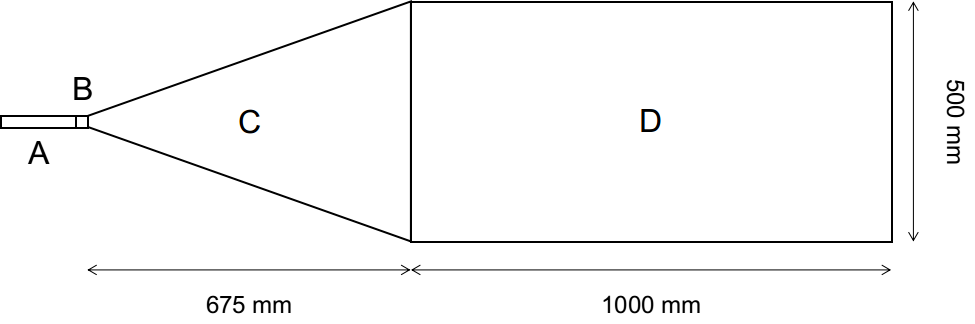
\includegraphics[width=0.75\columnwidth]{config.png}
	\caption{Schematic diagram of the HiSPARC scintillation detector. (A): PMT; (B): light-guide adaptor; (C): light-guide; (D): scintillator.}
	\label{fig:HS_scintillator}
\end{figure}

The scintillator is made of a material consisting of polyvinyltoluene as the base, with anthracene as the fluor, and the emission spectrum peaks at a wavelength of 425~nm \citep{fokkema_hisparc_2012, bartels_hisparc_2012}. The light-guide is made from \gls{pmma} and has a comparable refractive index to the scintillator (1.58 and 1.49, respectively), reducing refraction effects between the two materials \citep{van_dam_hisparc_2020}.

The \gls{pmt} used is an ETEnterprises 9125B model, with a 25~mm aperture,  blue-green sensitive bialkali photocathode, and 11 high-gain dynodes \citep{bartels_hisparc_2012,et_enterprises_data_2020}. The quantum efficiency of the \gls{pmt} used in the \gls{hisparc} detectors peaks at around 375~nm at 28\%, and at 425~nm the quantum efficiency is 25\% \citep{fokkema_hisparc_2012}. 

Each detector is wrapped in aluminium foil (thickness 30~$\upmu$m) and a black, vinyl material (thickness 0.45~mm), which is usually used as a pond liner, to ensure light-tight detectors and to reduce the noise level from stray photons \citep{van_dam_hisparc_2020}. In addition, each detector is placed inside of its own a plastic roof box to again ensure that it is light-tight, and to also ensure that it is weather-proof, as the detectors are usually located on the roofs of schools, colleges, and universities.

The \gls{hisparc} detectors have, individually, a high muon-detection
efficiency close to $100\%$ \citep{fokkema_hisparc_2012, van_dam_hisparc_2020}, therefore they are capable of observing any muons that traverse them. A \gls{hisparc} station combines either 2 or 4 detectors, to observe coincident muons (`events'), and typical configurations of each are shown in Figure~\ref{fig:HS_station_layouts}. The separation between detectors varies from station-to-station and this influences the measurable footprint and hence the observable \glspl{pcr}.


\begin{figure}[htbp!]
	\centering
	\subfloat[Two-detector station configuration]{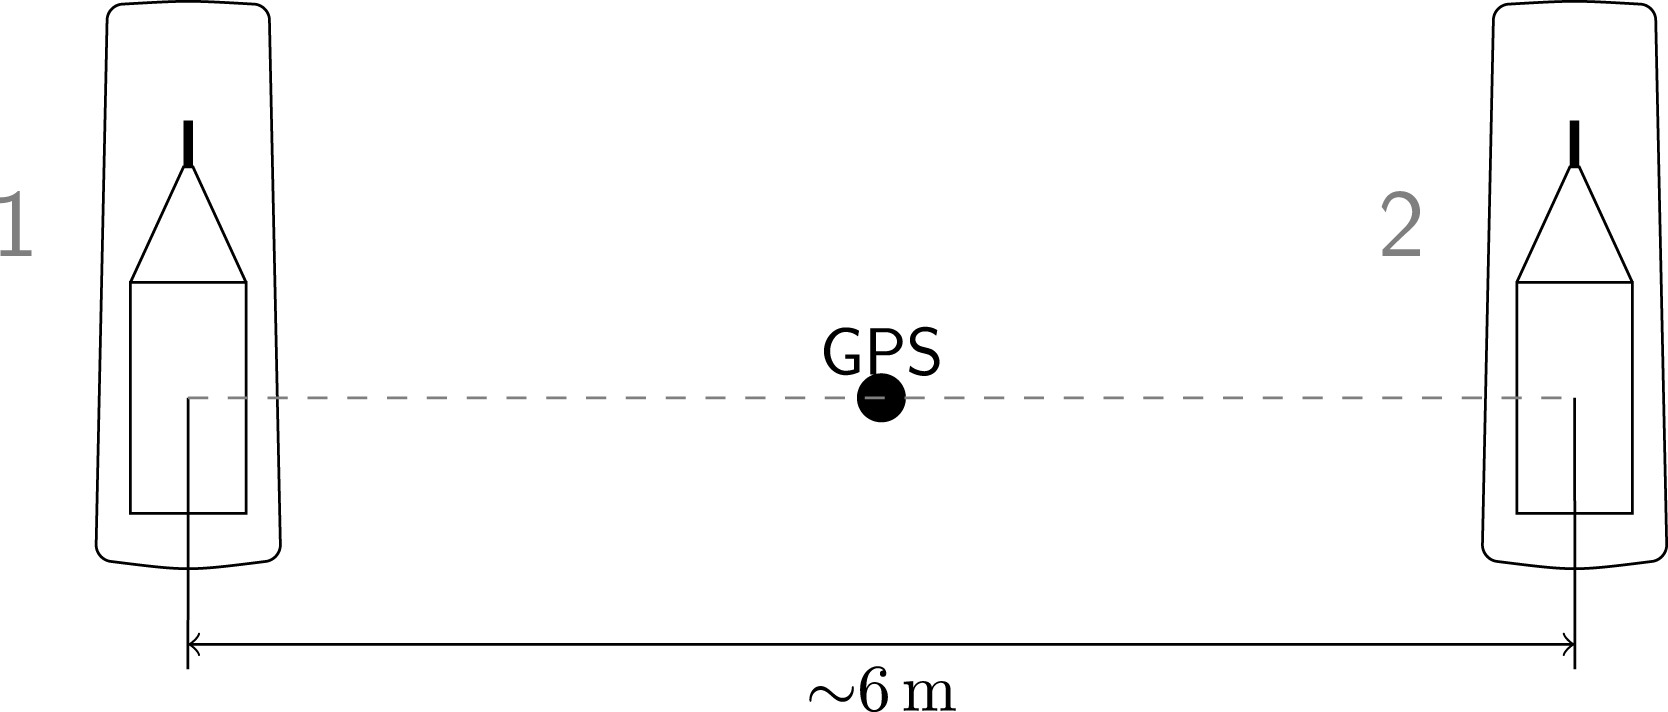
\includegraphics[width=0.5\columnwidth]{HS_2det.jpg}} 
	\qquad
	\subfloat[Four-detector station configuration (triangle arrangement)]{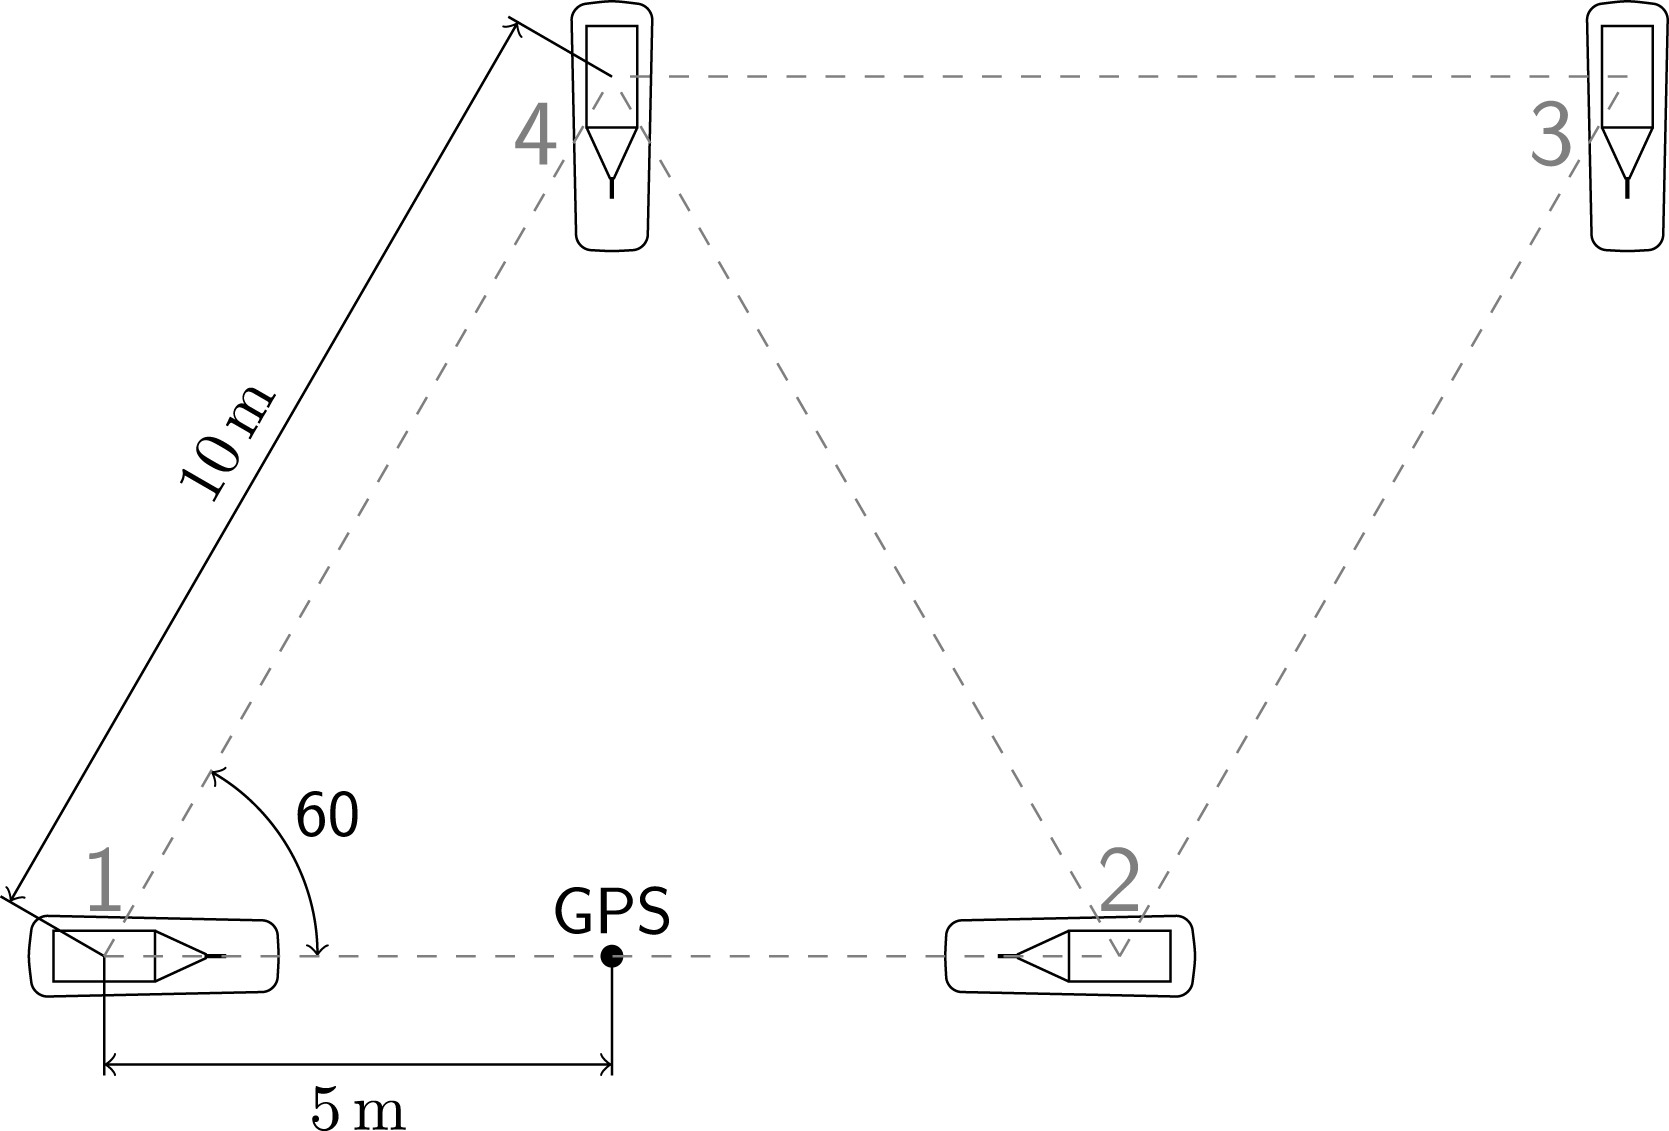
\includegraphics[width=0.5\columnwidth]{HS_4det-r.jpg}}
	\qquad
	\subfloat[Four-detector station configuration (diamond arrangement)]{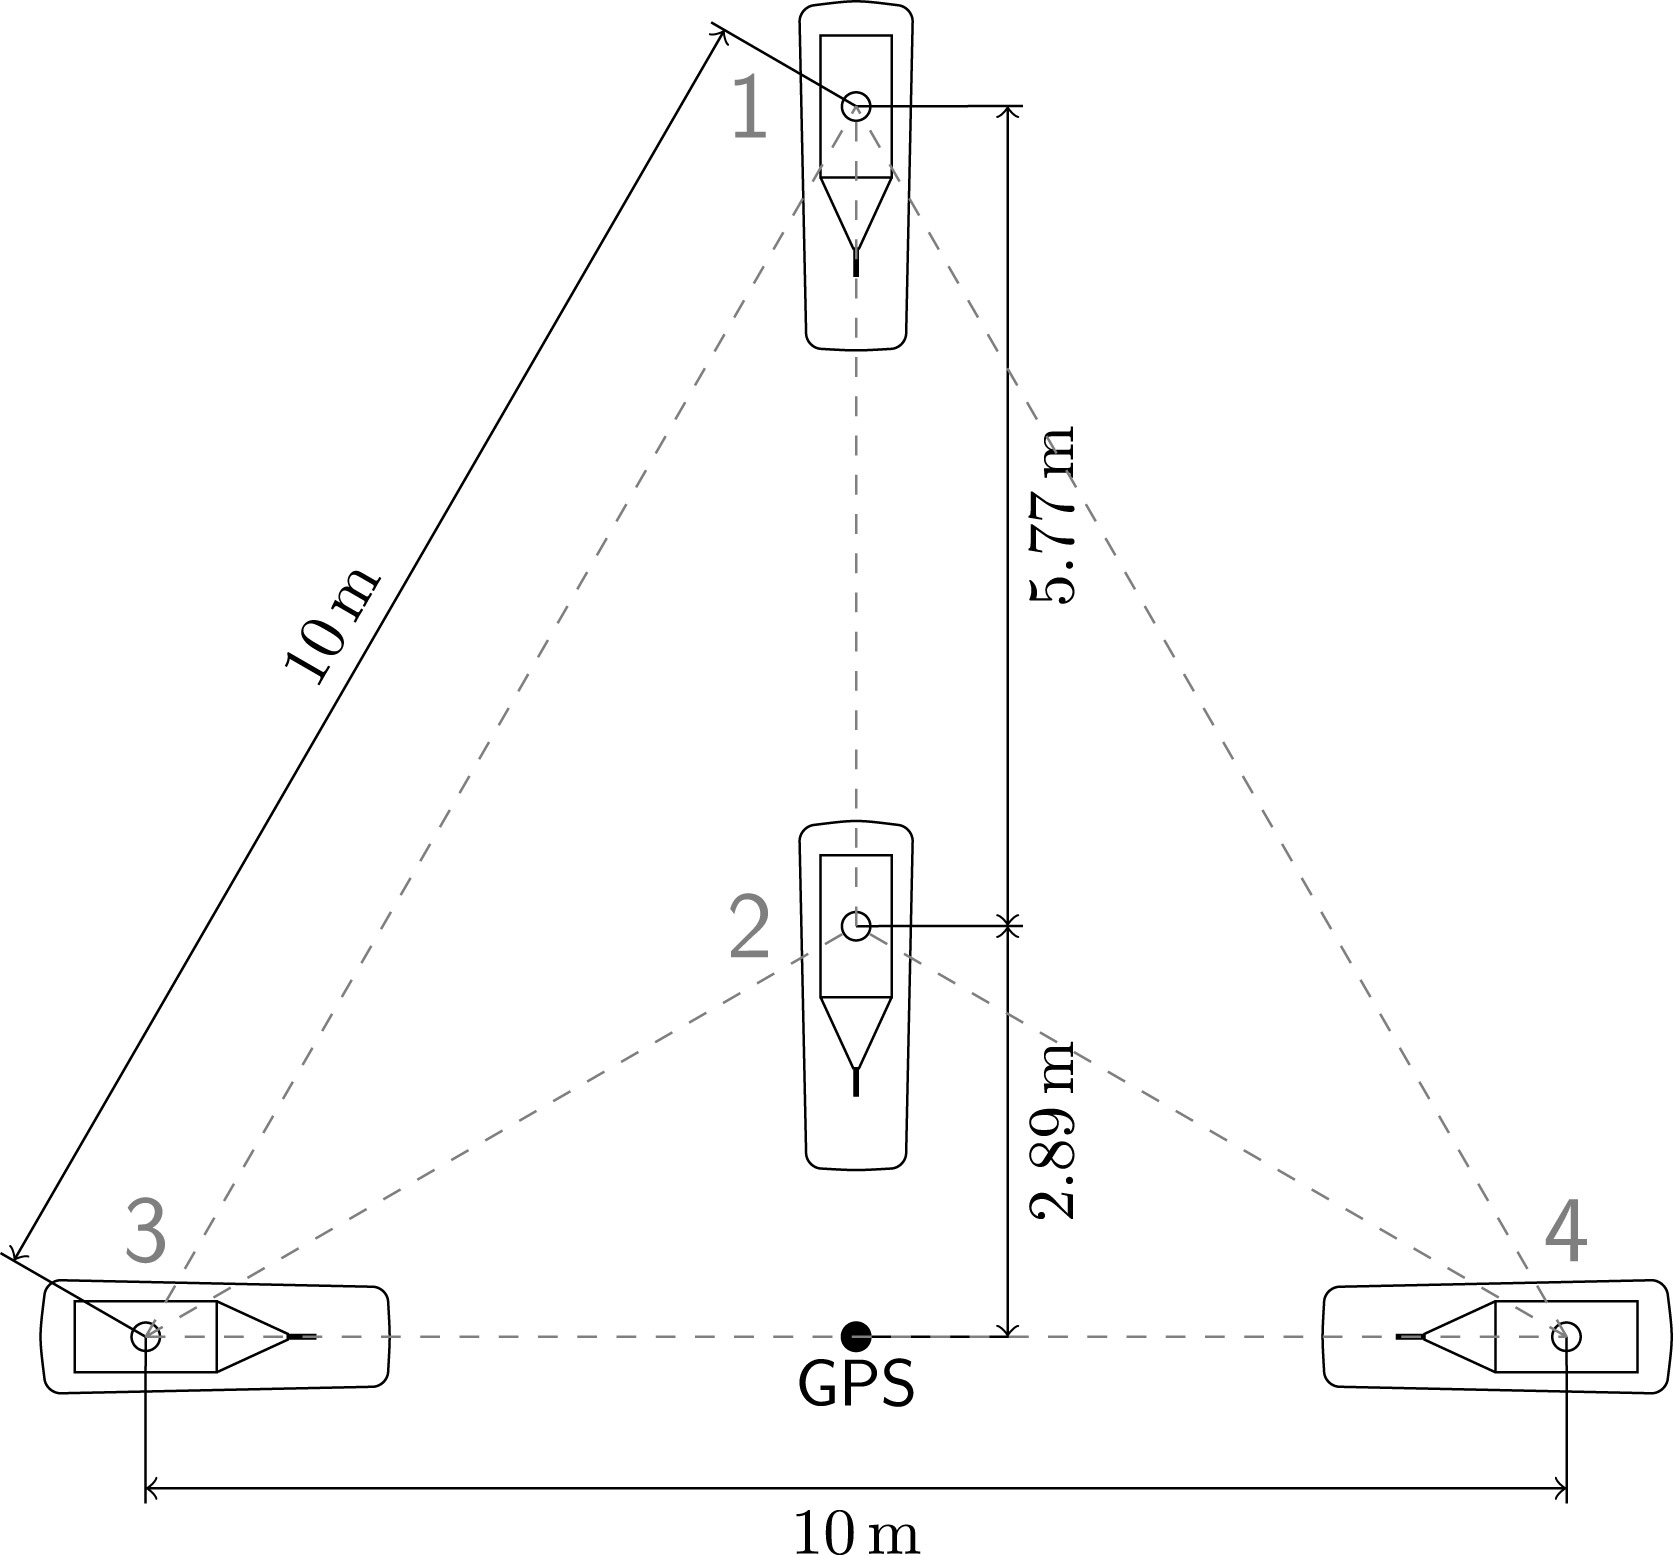
\includegraphics[width=0.5\columnwidth]{HS_4det-d.jpg}}
	\caption{Typical formations of two-detector and four-detector stations \citep{fokkema_hisparc_2012, van_dam_hisparc_2020}. In each, the black circle denotes a GPS antenna which is located in between the detectors to provide a precise timestamp for each signal.}
	\label{fig:HS_station_layouts}
\end{figure}


Furthermore some stations have the capability to measure the local atmospheric properties, such as temperature, pressure, relative humidity etc. Moreover, some stations also record the `singles' rates, i.e. the frequency at which an individual detector is triggered, independently of the other detectors in the station. The singles rates are important when investigating non-\gls{eas} events.

The scientific goals that can be achieved also vary between the two- and four-detector stations. When at least three detectors in a four-detector station observe particles of an \gls{eas}, the direction of the \gls{eas} (and thus the direction of the \gls{pcr}) can be acquired using triangulation calculations. When only two detectors in a station observe particles of an \gls{eas} it is only possible to reconstruct the arrival direction along the axis that connects the centres of those two detectors (thus it is not possible to reconstruct the direction of the \gls{pcr}).

The \glspl{pmt} of the detector in a station are connected to a \gls{hisparc} electronics box, which samples and digitises the signal at a rate of 400~MHz, and each \glspl{pmt} is connected to the electronics box using cables of a standard length of 30~m, to minimise any timing offsets between detectors \citep{fokkema_hisparc_2012, van_dam_hisparc_2020}. A schematic diagram showing the configuration of, and interfaces between, the \gls{hisparc} hardware is shown in Figure~\ref{fig:HS_hardware_config}. The electronics boxes are capable of controlling and reading two \glspl{pmt} (see Fig.~\ref{fig:HS_hardware_config}), therefore a four-detector station requires two electronics boxes: a primary and a secondary.


\begin{figure}[ht!]
	\centering
	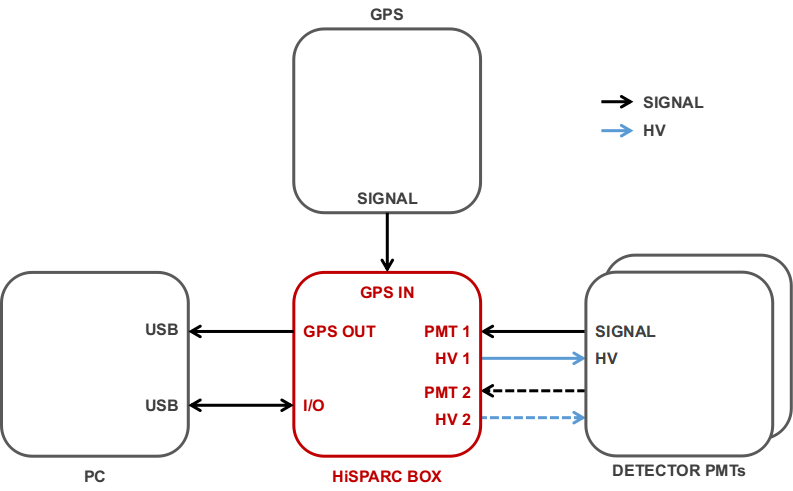
\includegraphics[width=\columnwidth]{HS_hardware_config.png}
	\caption{A schematic diagram showing the configuration and interfaces between the HiSPARC hardware for a two-detector station.}
	\label{fig:HS_hardware_config}
\end{figure}

Figure~\ref{fig:HS_hardware_config} shows all the hardware interfaces with the \gls{hisparc} electronics box, which communicates with the PC via USB. There are two connections for each \gls{pmt}, one for the control (i.e. \gls{hv}) and another for the signal. In addition, a \gls{gps} antenna is located in between the detectors in the station (shown in Fig.~\ref{fig:HS_station_layouts}). The \gls{hisparc} electronics box contains a \gls{gps} board, which provides an accurate timestamp for the data \citep{fokkema_hisparc_2012}.



%%%%%%%%%%%%%%%%%%%%%%%%%%%%%%%%%%%%%%%%%%%%%%%%%%%%%%%%%%%%%%%%%%%%%
\subsection{HiSPARC Data Acquisition}

\gls{hisparc} \gls{daq} software is used to control and read-out from the \gls{hisparc} electronics box. The \gls{daq} software was developed using LabVIEW, to be executed on a Windows PC \citep{van_dam_hisparc_2020}. Figure~\ref{fig:HiSPARC_trace} shows the typical output signal from one of the \glspl{pmt}, recorded by the \gls{daq} software. The depth of the trace is called the \textit{pulse height} and the area under the curve, the \textit{pulse integral}. The pulse integral is a measure of the number of scintillation photons that have arrived at the \gls{pmt}, exceeding the noise threshold ($-10$~mV) \citep{van_dam_hisparc_2020}. The \gls{hisparc} \gls{daq} software determines a signal baseline of the \gls{pmt} (i.e. the background signal without an incident muon), the pulse height, and pulse integral.

\begin{figure}[ht!]
	\centering
	\subfloat[Trigger pulse]{
		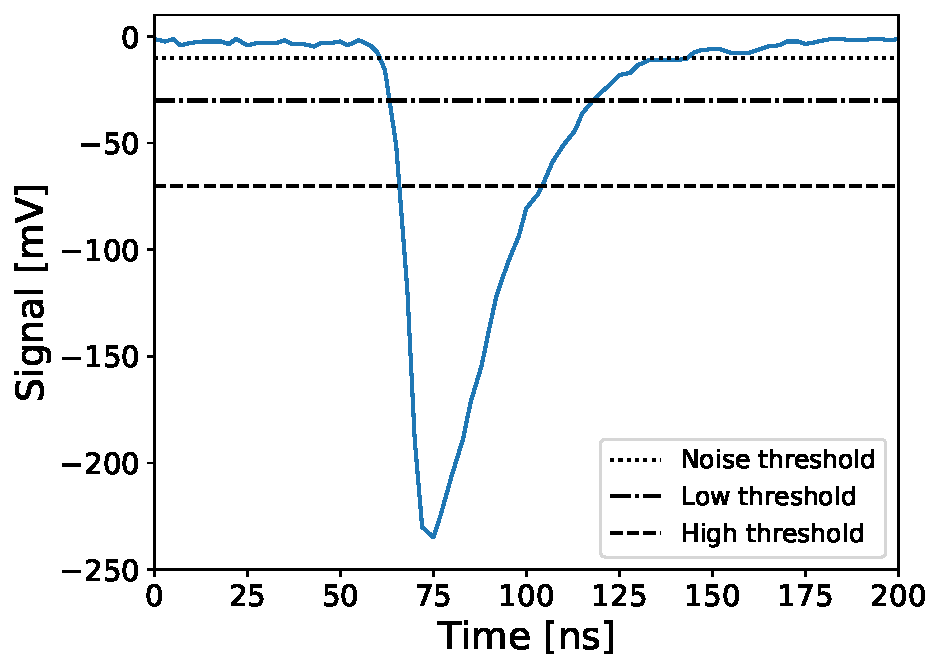
\includegraphics[width=0.48\columnwidth]{trace_plot.pdf}
		\label{fig:HiSPARC_trace}}
	%\qquad
	\subfloat[Pulse height spectrum]{
		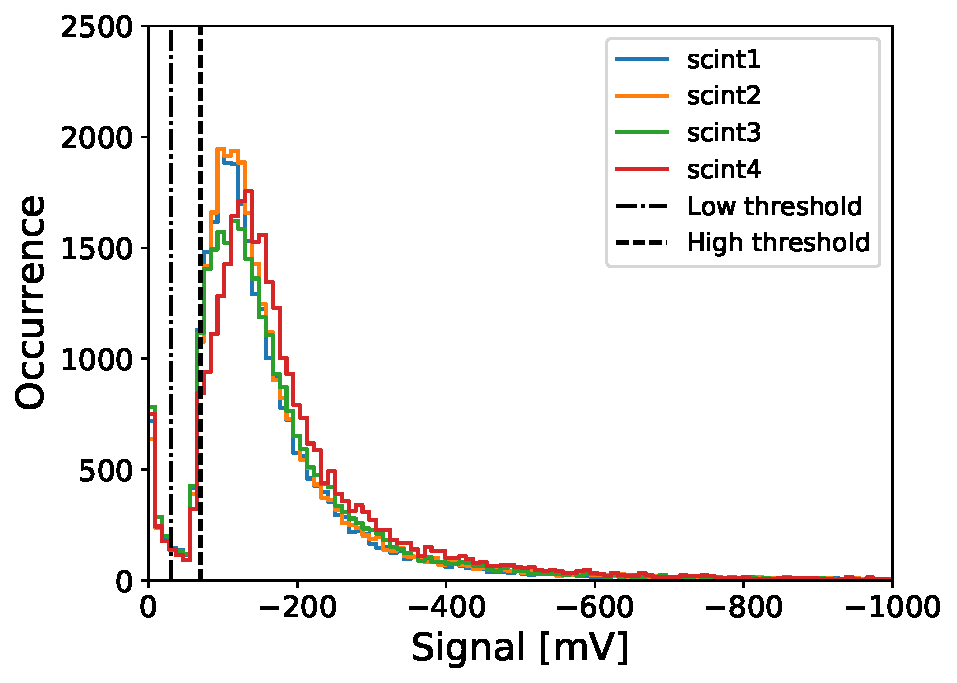
\includegraphics[width=0.48\columnwidth]{pulseheights.pdf}
		\label{fig:HiSPARC_pulseheight}}
	
	\caption{(a): An example PMT signal after digital conversion by the HiSPARC electronics box. The horizontal lines denote: the noise cut-off (dotted line), which is used for setting a limit when integrating the pulse height, to give the pulse integral; the low-voltage threshold (dash-dot); the high-voltage threshold (dashed). The role of the high- and low-voltage thresholds are described in the text below. (b) The pulse height distribution over the course of a single day from HiSPARC station 501. The vertical lines show the low-voltage threshold (dash-dot) and the high-voltage threshold (dashed).}
	\label{fig:pulses}
\end{figure}

The pulse height spectrum (see Figure~\ref{fig:HiSPARC_pulseheight}) is a histogram of all the pulses recorded by a detector. It is composed of two main regions: the left side which falls off rather steeply, and the main, asymmetric part of the spectrum which features a peak and a long tail. The left side of the spectrum is understood to be from high-energy photons (gamma rays) produced in air showers \citep{fokkema_hisparc_2012}. These high-energy photons may undergo pair production when interacting with the scintillator which may produce ionising electron and positron pairs.

The main, asymmetric distribution, which features a peak and a tail, is from charged particles (i.e. muons and electrons) \citep{van_dam_hisparc_2020}. The mean energy loss of particles in a material is described by the Bethe-Bloch formula; however this does not account for fluctuations in energy loss and a Landau distribution describes the fluctuations in energy loss of particles \citep{fokkema_hisparc_2012}. Due to the resolution of the \gls{hisparc} detectors the distribution in Figure~\ref{fig:HiSPARC_pulseheight} is best described by the convolution of the Landau distribution and a normal distribution which describes the resolution of the detector \citep{fokkema_hisparc_2012}. The peak of the distribution, the \gls{mpv}, is the most likely energy lost by a particle in the detector, i.e. the 3.51~MeV \citep{van_dam_hisparc_2020}. It has been shown that the location of the \gls{mpv} can vary due to the effects of atmospheric temperature \citep{bartels_hisparc_2012, van_dam_hisparc_2020}.

For each \gls{pmt}-channel, two discriminator thresholds can be defined: low- and high-voltage, as shown in Figure~\ref{fig:HiSPARC_pulseheight}, as vertical dash-dot and dashed lines, respectively.  The trigger thresholds are placed to reject the noise signals from the data, i.e. the left side of the pulse height spectrum. If a signal exceeds the high threshold, there is a high probability that the signal was generated by a particle in the detector. The `singles' data counts any time that the signal measured from a \gls{pmt} exceeds the low- or high-threshold.

The \gls{hisparc} experiment is configured in such a way as to ensure that each station across the \gls{hisparc} network measures a similar count rate of muons, in order to aid the direct comparison between the different stations in the network. When configuring the station, a trigger threshold must be applied for the \gls{pmt} signals. This is standardised across the \gls{hisparc} network and can be seen in relation to a detector trigger pulse in Figure~\ref{fig:HiSPARC_trace}. There are two thresholds, low: $-30$~mV, which represents $\sim0.2$ of a \gls{mip}; high: $-70$~mV, which represents $\sim0.5$ of a \gls{mip} \citep{fokkema_hisparc_2012, van_dam_hisparc_2020}. \citet{van_dam_hisparc_2020} states the thresholds were chosen to increase the sensitivity for observing gamma rays and low-energy electrons; the sensitivity is lower than for muons. However, as the detectors can measure gamma rays and electrons, it can be difficult to determine whether an individual detection was a muon, or another \gls{mip}, which is why the \gls{hisparc} network usually relies on detecting `events', from coincident muons.

To register an `event', the detectors must measure signals which exceed the low threshold, within a limited time window. The time-line of the data acquisition during an event is given in Figure~\ref{fig:HS_windows}.

\begin{figure}[ht!]
	\centering
	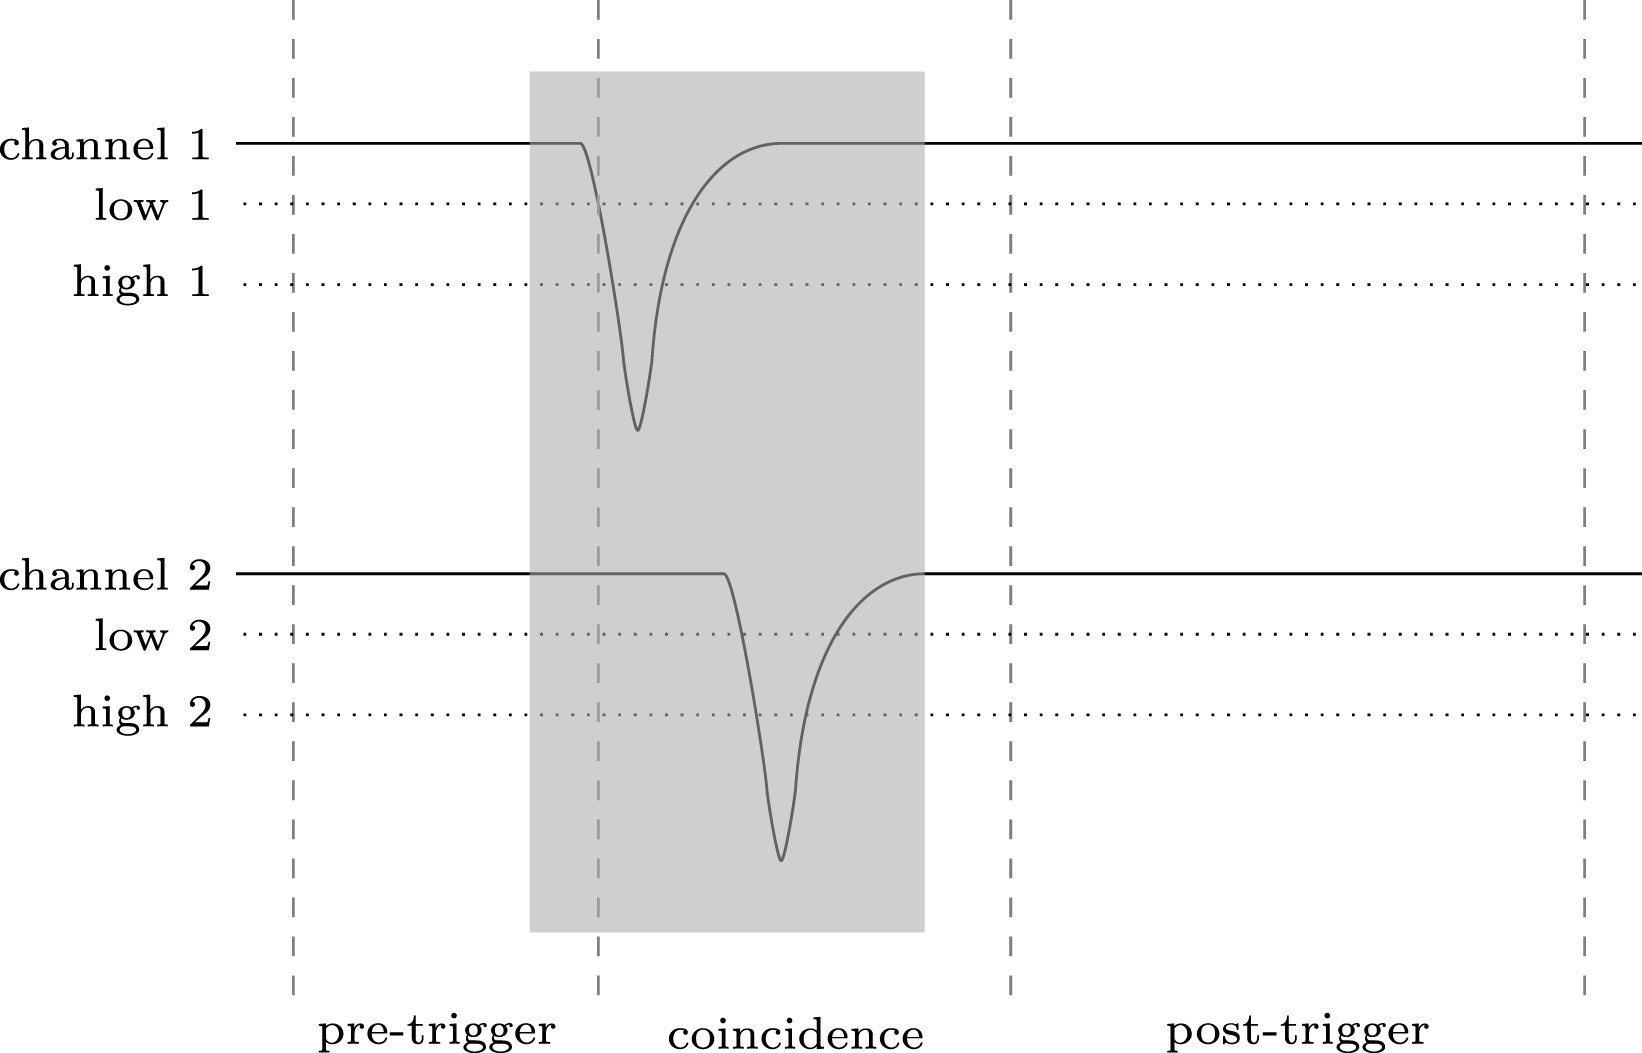
\includegraphics[width=0.9\columnwidth]{HS_pulses.jpg}
	\caption{Schematic diagram of the time-line for the data acquisition of an event \citep{fokkema_hisparc_2012}. The dashed vertical lines denote the epochs of the pre-trigger, coincidence, and post-trigger windows. The grey, shaded region shows the data reduction window and data outside this window are not stored. The dotted, horizontal lines denote the low- and high-voltage thresholds.}
	\label{fig:HS_windows}
\end{figure}

When channel~1 (i.e. \gls{pmt}~1) exceeds the low-threshold a coincidence window is opened. The length of the coincidence window is $\sim1.5~\upmu\mathrm{s}$. If, within this window, channel~2 (i.e. \gls{pmt}~2) also measures a signal that exceeds the low threshold, the trigger condition is met and an event is generated. When a trigger is issued, the output is stored in the buffer of the \gls{fpga} in the \gls{hisparc} electronics box \citep{fokkema_hisparc_2012}. The data acquisition software reads the data from the buffer and the full event data consist of: (i) data measured before the coincidence window was opened (the pre-trigger window, typical length $\sim1~\upmu\mathrm{s}$); (ii) data measured within the coincidence window; (iii) data measured after the trigger period (the post-trigger window, typical length $\sim3.5~\upmu\mathrm{s}$). Therefore the event window lasts for $\sim6~\upmu\mathrm{s}$ in total, with the maximum length of an event window of $10~\upmu\mathrm{s}$ \citep{van_dam_hisparc_2020}. Finally, a data reduction algorithm is applied on the full event window which determines the part of the signal containing the muon pulses---compared to the baseline---and removes the rest, thus greatly reducing the size of the event data \citep{fokkema_hisparc_2012}.
%algorithm determines the part of the signal containing the PMT pulses and removes the res


The default trigger condition for detecting an air shower event between multiple \glspl{pmt} within a station differs for a two- and four-detector station. In a two-detector station, an event is recorded if the \gls{pmt} signals from both detectors exceed the low threshold within the coincidence time window ($1.5~\upmu\mathrm{s}$). In a four-detector station, the default trigger condition is either: (i) at least two detectors exceed the high threshold within the coincidence time window; (ii) at least three detectors exceed the low threshold within the coincidence time window. These are the default conditions, but there are other, user configurable ways of triggering the station.


%Each detector in the network is set up such that the pulse height spectrum peaks at a \gls{mpv} of $\sim 150$~mV (see Figure~\ref{fig:pulses}), and such that the high threshold allows a mean count rate on the order 100 counts per second and the low threshold allows a mean count rate of the order 400 counts per second; these can by tuned by adjusting the \gls{pmt} voltage. It could be argued that in setting up the detectors in this way, there is an immediate bias in the data to reject lower energy \glspl{cr}.


Data recorded by the \gls{hisparc} stations are stored and are available on the \gls{hisparc} Public Database\footnote{\url{https://data.hisparc.nl/}}, where each station is listed, grouped by local nodes. For every station one can see its ID, name, and a coloured square and circle displaying its current data delivery and \gls{daq} status, respectively. Clicking on any station takes you to a dedicated page which displays its data on a user-selected day. Where data are available, it is possible to download: %The data are stored in {\verb HDF5 } format but are downloaded in {\verb .tsv } format.
%
\begin{itemize}
	\item{events rate data: where multiple detectors in a station are triggered to satisfy that station's trigger condition;}
	\item{singles rate data: the count rates of the individual detectors within a station;}
	\item{weather data: meteorological data, including pressure and temperature;}
	\item{coincidences data: the counts where different stations measure the same event (to within $1.36 \, \upmu$s); it is possible to determine if stations measured the same event by comparing the \gls{gps} timestamps of events.}
\end{itemize}

To support the \gls{hisparc} project, the \gls{sapphire} Python package \citep{fokkema_hisparc_2012,fokkema_sapphire_2012} was written. This Python package provide a framework to analyse the \gls{hisparc} data, but also an alternative way to acquire the data.



%To discriminate against single particle sources, \gls{hisparc} applies the ’coincidence method’. By using two (or four) detectors and selecting coincident PMT pulses (i.e. with a time difference smaller than 1.5 µs) the majority of random coincidences are rejected. If two or more PMT pulses exceed the threshold within the trigger window, the pulses are stored




\glsresetall 
{}
%%%%%%%%%%%%%%%%%%%%%%%%%%%%%%%%%%%%%%%%%%%%%%%%%%%%%%%%%%%%%%%%%%%%%%%%
%%%%%%%%%%%%%%%%%%%%%%%%%%%%%%%%%%%%%%%%%%%%%%%%%%%%%%%%%%%%%%%%%%%%%%%%
%%%%%%%%%%%%%%%%%%%%%%%%%%%%%%%%%%%%%%%%%%%%%%%%%%%%%%%%%%%%%%%%%%%%%%%%
\section{Thesis Structure}

In this thesis a number of projects are presented which explore the themes of understanding the solar interior-atmosphere linkage and space weather applications. This is broken down into three major projects: a feasibility study on \gls{cr} space weather applications, an investigation into the effects of solar activity on \gls{cr} observations, and a study of the \gls{smmf}. The thesis is structured as follows:
%To clarify the structure of this thesis, the contents of each chapter and the main themes within are given in outline, before I present the work in each.

In Chapter~\ref{chap:HiSPARC} we perform a feasibility study to determine whether the \gls{hisparc} network is suitable for monitoring space weather events. This was achieved using historic data from the \gls{hisparc} network to search for the signature of space weather events. In addition we performed simulations of \glspl{as} to determine the expected variation in muon counts during space weather events. At the time of writing, the work in this chapter had not been published in any journals.

Following the results of Chapter~\ref{chap:HiSPARC}, Chapter~\ref{chap:HiSPARC_14008} outlines the design of an alternative \gls{hisparc} station, with a novel arrangement of detectors that removes thermally induced, diurnal variations in the data, and reduces the existing energy bias of observable \glspl{pcr} using the \gls{hisparc} network. In this chapter we discuss the set-up of the station, review the data and its noise properties, and finally also perform simulations using artificial data to investigate the capabilities of this new configuration. At the time of writing, the work in this chapter had not been published in any journals.

In Chapter~\ref{chap:GCR_SSN_24} we studied long-term variations of \gls{gcr} intensity in relation to the \gls{ssn} during the most recent solar cycles. This study, which was published in the journal Solar Physics \citep{ross_behaviour_2019}, analysed the time lag between the \gls{gcr} intensity and the \gls{ssn}, and the hysteresis effect of the \gls{gcr} count rate against \gls{ssn} for Solar Cycles 20--24..

Chapter~\ref{chap:SMMF} presents a frequency-domain analysis of over 20~years of high-cadence \gls{bison} observations of the \gls{smmf} is presented. We modelled the power spectrum of the \gls{bison} \gls{smmf} data to draw conclusions about the morphology of the \gls{smmf}, particularly focusing on the source of the rotationally modulated component in the signal. A significant portion of the work presented in this chapter was published in the journal Monthly Notices of the Royal Astronomical Society \citep{ross_lifetimes_2021}.

In Chapter~\ref{chap:rmode} we further investigated the \gls{bison} \gls{smmf} data. Here we examined the residual spectrum, after removing our best-fitting model, to search for evidence of a magnetic signature of global Rossby modes ($r$ modes). At the time of writing, the work in this chapter had not been published in any journals.

All of the results presented in the chapters of this thesis are my own and all the data analysis was performed by me. Input from others came only in the form of advice and consultation, in addition to the supply of raw data.

Finally, the thesis is concluded in Chapter~??.